\documentclass[12pt,letterpaper]{article}
\usepackage{graphicx}
\usepackage{nomencl}
\usepackage{subfigure}
\usepackage{subfigmat}
\usepackage{amssymb}
\usepackage{mathtools}
\usepackage{rotating}
\usepackage{placeins}%Enables \FloatBarrier, a tag across which floats
                     %(figures, tables, etc.) may not pass.
\usepackage{booktabs}%For professional tables
\usepackage{draftcopy}%Draft watermark
\usepackage{array}
\usepackage{wrapfig}
%\usepackage{mdwlist}
\makenomenclature
%\usepackage{amsmath}
\title{Comprehensive Exam Proposal}
\author{C.~Nathan Woods}
% \degree{Doctor of Philosophy}
% \otherdegrees{B.S. Physics, Brigham Young University, 2008}
% \dept{Department of}{Aerospace Engineering Sciences}
% \advisor{}{Dr.~Ryan Starkey}
% \abstract{ \OnePageChapter This is an abstract test}
% \dedication{Dedication}
% \acknowledgements{ \OnePageChapter Acknowledgements}
% % Commented out for multiple page ToC
% %\ToCisShort % a 1-page Table of Contents 
% \LoFisShort % a 1-page List of Figures
% %\emptyLoF % no LoF
% \LoTisShort % a 1-page List of Tables
% %\emptyLoT % no LoT

\begin{document}
\maketitle
\begin{abstract}
Computational fluid dynamics, or CFD, has tremendous potential for
applications in high-speed-vehicle design, but this potential has been
unrealized due to the high initial costs, both human and computational,
of CFD simulations. The purpose of this work is to use W. H. Hui's unified
coordinate system to craft an accurate, efficient, two-dimensional CFD
program for compressible aerodynamics with complex geometries. This
program will combine routines for inviscid flow with boundary-layer
techniques and Navier-Stokes solvers to reduce computational costs
using a stream-oriented, moving grid framework
developed by Hui.
\end{abstract}
\tableofcontents
\listoffigures
\printnomenclature
\section{Introduction}
Computational fluid dynamics, or CFD, dramatically altered the field
of aerodynamics during the twentieth century, and continues to be an
essential part of aerodynamic analysis around the world, both as a
supplement to wind-tunnel testing and as a replacement when
circumstances require. Unfortunately, CFD is not without its costs,
especially for design work. To quote Jameson, 
``CFD is still not being exploited as effectively as one 
would like in the design process. This is partially 
because of the long set-up times and high costs, both 
human and computational, of complex flow simulations."\cite{jameson97}

Automatic grid generation for complex problems
would greatly reduce the set-up time and human costs, and good
progress has been made on this front using unstructured
grids. However, structured grids, which offer significant advantages
in terms of memory use, grid adaptation, and algorithm maturity (see
\cite{steinthorsson95}\cite{boeing05}\cite{badcock00} and
\cite{IDAreview05}), they have so far resisted automation. 

W.H Hui et al developed and demonstrated a method of automatic,
structured, grid generation using a time-dependent grid whose motion
was a function of the local fluid velocity. 
The grid is generated at the upstream boundary and allowed to flow
through the simulation region until it fills the area of interest.
The actual grid motion is completely specified by
requiring the grid velocity to preserve some quantity of interest,
such as skewness or jacobian. This eliminates the major
problems of skewness and arbitrarily small
jacobian\cite{venkatakrishnan95} associated with grid-point-movement
methods of solution-adaptive grid refinement, while simultaneously
yielding the excellent resolution of slip lines that is characteristic
of a streamline-oriented grid.


% Computing a fluid-dynamical solution for a complicated flow problem 
% can be slow, the equations solved are only approximations to the 
% actual physical system, and every simulation must start with a 
% computational mesh, the form of which can drastically affect overall 
% solution accuracy and computational efficiency. Because of these 
% limitations, CFD remains largely the province of highly trained 
% professionals and academics, whose education and experience are 
% integral in obtaining accurate results.

% The dependence of CFD simulations on the computational mesh used is 
% particularly troubling, as a mesh generated by an unskilled user can 
% produce highly erroneous results. This problem has spawned decades of 
% study, and many good methods for generating these meshes have been 
% found, but most of these methods require active participation and 
% understanding from the user. For a complicated flow that must be 
% resolved with a high degree of certainty, generation of the mesh can 
% take weeks, even months. As a result, accurate CFD has been limited to 
% applications where the up-front costs of mesh generation by competent 
% specialists are justified.

% Unfortunately, those applications do not include early-stage projects 
% and preliminary design work. When simulation boundaries regularly 
% change, as is common during the early stages of vehicle design, each 
% change necessitates the generation of a new mesh, the costs of which 
% rapidly outweigh the benefits CFD simulations provide. As a result, 
% critical design decisions are made without the highly relevant 
% aerodynamic information that CFD can provide, and bad decisions made 
% early on can be very difficult to undo later.

% The goal of this current work is to enable the generation of
% reasonably accurate solutions 
% to complex flow problems at low user-involvement and low computational 
% cost. The Unified Coordinate System (UCS) defined by 
% W. H. Hui\cite{hui07} shows promise in this area, but its 
% characteristics have never been fully explored and documented. In this 
% paper, we present the results of a formal grid-convergence study on 
% the original implementation of the UCS method\cite{hui99}. We further 
% characterize its behavior, which will provide direction to those 
% looking to use UCS in their projects. Several interesting test cases 
% are also presented to further highlight the utility of the method.

Although much has been done to develop Hui's methods in various
situations, no one has ever assembled the disparate prototype solvers
into a coherent whole. The goal of this project is to craft a powerful
new design tool by assembling the different ideas into a complete
package that will automatically and quickly compute fluid flows under
arbitrary conditions. 

For instance, consider the solution of flow around the Space
Shuttle. It consists of a largely supersonic flow region, with a very
tight and highly reactive shock and boundary layer around the leading
edge of the vehicle, and a powerful wake downstream. The ideal
situation would be to accept a (perhaps 
time-dependent) geometric definition of the Shuttle's aerodynamic
shape and compute, without user intervention, a steady supersonic
solution wherever possible, and subsonic, ionized, reactive, and
time-dependent bubbles wherever necessary, without 
generating a body-fitted grid. Unfortunately, such a solver has been
the target of decades of research without full success. 
% Talk about verification; it's brand-new in terms of publication, and
% the basis of one of my journal papers
The goal of
this dissertation will be a subset of the ideal situation, combining
the following solvers in an 
automatic way for two-dimensional flows:
\begin{itemize}
\item A time-marching Euler solver to handle general inviscid flows.
\item A boundary-layer equation solver to introduce
  viscous effects for flows without separation.
\item A laminar Navier-Stokes solver to handle
  regions of separation and recirculation.
\item A steady-state, supersonic Euler solver to
  greatly reduce the time required for inviscid computation.
\end{itemize}
%Further discussion of these items and a specific timeline are outlined
%in Sec.~\ref{sec:timeline}.

% To leverage the work that has been done in the unified coordinate
% system into the creation of a powerful design tool that is light,
% fast, respectably accurate, and automatic.
% \subsection{Stitching and Patches}
% Base Euler Flow
% Space-marching supersonic
% Time-marching subsonic
% Stationary mesh (grid separation)
% Moving wall conditions
% Boundary-layer solution
% Thin boundary layers
% Minimal separation
% Massive separation
% Navier-Stokes equations
% Full separation regions with recirculation, etc.
% Turbulence models?
% Automated patch generation/stitching


\section{Background}
\label{sec:background}
\subsection{Hui and the Unified Coordinates}
The unified coordinate system arose from a series of studies that 
used Lagrangian coordinates to clearly resolve slip lines in 
supersonic flows, and it is best understood in that context.
In the current implementation, 
grid points move in the same direction as the fluid, but at different
speeds. The additional freedom 
introduced by allowing the speed of the grid points to vary allows the simulation to 
capture many useful properties of the Lagrangian coordinate system,
such as automatic grid generation and excellent slip line resolution, 
while also maintaining a structured, regular (orthogonal, if the flow permits) 
grid. In particular, 
the grid follows fluid pathlines, automatically 
conforms to solid boundaries, and resolves slip lines nearly 
perfectly. It does this at the cost of requiring the dynamic creation 
and destruction of nodes at in- and out-flow simulation boundaries, 
and the computational costs associated with solving a linear, first 
order, ordinary differential equation in space at each time step. 

\subsubsection{Coordinate Transformations}
A generic, time-dependent, coordinate transformation in three 
dimensions can be written 
\begin{align}
\label{eq:coordinate_transformation}
\left(
\begin{array}{c}
dt\\dx\\dy\\dz
\nomenclature[]{$t$}{Time in physical space}
\nomenclature[]{$x$}{$x$ component of position in physical space}
\nomenclature[]{$y$}{$y$ component of position in physical space}
\nomenclature[]{$z$}{$z$ component of position in physical space}
\nomenclature[]{$\vec{x}$}{Vector of physical, cartesian coordinates,
  including $t$ as the $0^{th}$ component}
\end{array}
\right) &= \left(
\begin{array}{cccc}
1 & 0 & 0 & 0 \\
U & A & L & P \\
V & B & M & Q \\
W & C & N & R \end{array} \right)
\nomenclature[]{$U$}{$x$ component of grid velocity, equivalent to
  $\frac{\partial x}{\partial \tau}$}
\nomenclature[]{$V$}{$y$ component of grid velocity, equivalent to
  $\frac{\partial y}{\partial \tau}$}
\nomenclature[]{$W$}{$z$ component of grid velocity, equivalent to
  $\frac{\partial z}{\partial \tau}$}
\nomenclature[]{$A$}{Component of coordinate transformation, equivalent
  to $\frac{\partial x}{\partial \xi}$}
\nomenclature[]{$B$}{Component of coordinate transformation, equivalent
  to $\frac{\partial y}{\partial \xi}$}
\nomenclature[]{$C$}{Component of coordinate transformation, equivalent
  to $\frac{\partial z}{\partial \xi}$}
\nomenclature[]{$L$}{Component of coordinate transformation, equivalent
  to $\frac{\partial x}{\partial \eta}$}
\nomenclature[]{$M$}{Component of coordinate transformation, equivalent
  to $\frac{\partial y}{\partial \eta}$}
\nomenclature[]{$N$}{Component of coordinate transformation, equivalent
  to $\frac{\partial z}{\partial \eta}$}
\nomenclature[]{$P$}{Component of coordinate transformation, equivalent
  to $\frac{\partial x}{\partial \zeta}$}
\nomenclature[]{$Q$}{Component of coordinate transformation, equivalent
  to $\frac{\partial y}{\partial \zeta}$}
\nomenclature[]{$R$}{Component of coordinate transformation, equivalent
  to $\frac{\partial z}{\partial \zeta}$}
\left( \begin{array}{c}
d\tau\\d\xi\\d\eta\\d\zeta \end{array} \right).
\nomenclature[]{$\tau$}{Time in computational space}
\nomenclature[]{$\xi$}{Component of position in computational space}
\nomenclature[]{$\eta$}{Component of position in computational space}
\nomenclature[]{$\zeta$}{Component of position in computational space}
\nomenclature[]{$\vec{\xi}$}{Vector of computational coordinates,
  including $\tau$ as the $0^{th}$ component}
\nomenclature[]{$\vec{u}$}{Fluid velocity 4-vector, with $1$ as the
  $0^{th}$ component}
\nomenclature[]{$\vec{U}$}{Grid velocity 3-vector, with Cartesian
  components given by $U$, $V$, $W$}
\end{align}

Such a coordinate transformation could also be written more succinctly 
in index notation:

\begin{equation}
\label{eq:coordinate_transformation_index}
dx_\alpha=\frac{\partial x_\alpha}{\partial \xi^\beta} d\xi_\beta 
\nomenclature[]{$_{\alpha,\,\beta}$}{Summation index running from 0 to 3}
\nomenclature[]{$_{i,\,j}$}{Summation index running from 1 to 3}
\end{equation}

\noindent where $\frac{\partial x_\alpha}{\partial \xi^\beta}$ are the
components of the
transformation matrix given in
Eq.~\ref{eq:coordinate_transformation}. The derivatives transform
differently: 

\begin{equation}
\label{eq:derivative_transformation_index}
\frac{\partial} {\partial x^\alpha}=
\frac{\partial \xi_\beta} {\partial x^\alpha}
\frac{\partial} {\partial \xi^\beta}
\end{equation}

\noindent That is, the derivatives transform via the transpose of the inverse of
the matrix that transforms the differentials. 

\begin{align}
\label{eq:derivative_transformation}
\left(
\begin{array}{c}
\frac{\partial}{\partial t} \\[.5em] \frac{\partial}{\partial x} \\[.5em]
\frac{\partial}{\partial y} \\[.5em] \frac{\partial}{\partial z}
\end{array}
\right) &= \left(
\begin{array}{cccc}
1 & -U_\xi & -U_\eta & -U_\zeta \\[.5em]
0 & \frac{MR-NQ}{J} & \frac{CQ-BR}{J}  & \frac{BN-CM}{J}  \\[.5em]
0 & \frac{NP-LR}{J} & \frac{AR-CP}{J} & \frac{CL-AN}{J}  \\[.5em]
0 & \frac{LQ-MP}{J} & \frac{BP-AQ}{J} & \frac{AM-BL}{J} 
\end{array} \right)
\left( \begin{array}{c}
\frac{\partial}{\partial \tau} \\[.5em] \frac{\partial}{\partial \xi} \\[.5em]
\frac{\partial}{\partial \eta} \\[.5em] \frac{\partial}{\partial \zeta}
\end{array}
\right).
\end{align}

\noindent where we have:

\begin{equation}
\nomenclature[]{$J$}{Jacobian of the coordinate transformation}
J=\left|\begin{array}{ccc}
A&L&P\\
B&M&Q\\
C&N&R
\end{array}\right|
\end{equation}
\begin{align}
\nomenclature[]{$\nabla_{\vec{x}}$}{Gradient operator with respect to
  physical spatial coordinates}
\nabla_{\vec{x}}\xi&\equiv \frac{MR-NQ}{J},\frac{NP-LR}{J},\frac{LQ-MP}{J}\\
\nabla_{\vec{x}}\eta&\equiv \frac{CQ-BR}{J},\frac{AR-CP}{J},\frac{BP-AQ}{J}\\
\nabla_{\vec{x}}\zeta&\equiv \frac{BN-CM}{J},\frac{CL-AN}{J},\frac{AM-BL}{J}\\
\end{align}
\begin{align}
\nomenclature[]{$U_\xi$}{$\xi$ component of grid velocity, equivalent to
  $\frac{\partial \xi}{\partial t}$}
\nomenclature[]{$U_\eta$}{$\eta$ component of grid velocity, equivalent to
  $\frac{\partial \eta}{\partial t}$}
\nomenclature[]{$U_\zeta$}{$\zeta$ component of grid velocity, equivalent to
  $\frac{\partial \zeta}{\partial t}$}
U_\xi&\equiv\vec{U}\cdot\nabla_{\vec{x}}\xi\\
U_\eta&\equiv\vec{U}\cdot\nabla_{\vec{x}}\eta\\
U_\zeta&\equiv\vec{U}\cdot\nabla_{\vec{x}}\zeta
\end{align}

$U_\xi$, $U_\eta$, and $U_\zeta$ are the components of grid velocity
in the $\xi$, $\eta$, and $\zeta$ directions, respectively. 
From Eq.~\ref{eq:coordinate_transformation}, we can also show

\begin{equation}
\label{eq:moving_computational_cells}
\frac{D_{\vec{U}}}{Dt}
\left(
\begin{array}{c}\xi\\\eta\\\zeta\end{array}
\right)=0
\end{equation}
\nomenclature[]{$\frac{D_{\vec{U}}}{Dt}$}{Material derivative with
  respect to grid velocity $\vec{U}$}
\noindent where $\frac{D_{\vec{U}}}{Dt}\equiv\frac{\partial}{\partial
  t}+\vec{U}\cdot\nabla_{\vec{x}}$. Therefore, the transformed
coordinates move with velocity $\vec{U}$.

Eq.~\ref{eq:coordinate_transformation} introduces 12 new variables,
but they are not all independent. In order for the coordinate
transformation to be single-valued, the coordinate differentials 
$d\xi_\alpha$  must be exact.\cite{hui99} This is equivalent to requiring that 
each differential be expressible as the exterior derivative $d$ of 
some scalar function $f$. For $d\xi$, this could be written:

\begin{equation}
d\xi = df = \frac{\partial f}{\partial \xi^\alpha}d\xi_\alpha
\end{equation}

Similar equations hold for $\eta$ and $\zeta$. This implies that by differentiating $df$ and using the requirement
that mixed partial derivatives commute, any exact differential must
satisfy the compatibility conditions:

\begin{equation}
\label{eq:compatibility_conditions}
\frac{\partial^2 x_\alpha}{\partial \xi^\alpha \partial \xi^\beta} =
\frac{\partial^2 x_\alpha}{\partial \xi^\beta \partial \xi^\alpha}\Rightarrow
\left\{
\begin{array}{ccc}
\frac{\partial A}{\partial \tau} = \frac{\partial U}{\partial \xi} &
\frac{\partial B}{\partial \tau} = \frac{\partial V}{\partial \xi} &
\frac{\partial C}{\partial \tau} = \frac{\partial W}{\partial \xi} \\[.5em]
\frac{\partial L}{\partial \tau} = \frac{\partial U}{\partial \eta} &
\frac{\partial M}{\partial \tau} = \frac{\partial V}{\partial \eta} &
\frac{\partial N}{\partial \tau} = \frac{\partial W}{\partial \eta} \\[.5em]
\frac{\partial P}{\partial \tau} = \frac{\partial U}{\partial \zeta} &
\frac{\partial Q}{\partial \tau} = \frac{\partial V}{\partial \zeta} &
\frac{\partial R}{\partial \tau} = \frac{\partial W}{\partial \zeta}
\\[.3em]
 &  & \\[.3em]
\frac{\partial A}{\partial \eta} = \frac{\partial L}{\partial \xi} &
\frac{\partial B}{\partial \eta} = \frac{\partial M}{\partial \xi} &
\frac{\partial C}{\partial \eta} = \frac{\partial N}{\partial \xi} \\[.5em]
\frac{\partial A}{\partial \zeta} = \frac{\partial P}{\partial \xi} &
\frac{\partial B}{\partial \zeta} = \frac{\partial Q}{\partial \xi} &
\frac{\partial C}{\partial \zeta} = \frac{\partial R}{\partial \xi} \\[.5em]
\frac{\partial L}{\partial \zeta} = \frac{\partial P}{\partial \eta} &
\frac{\partial M}{\partial \zeta} = \frac{\partial Q}{\partial \eta} &
\frac{\partial N}{\partial \zeta} = \frac{\partial R}{\partial \eta} 
\end{array}
\right.
\end{equation}

It is important to note that these compatibility conditions are not
independent either. The first nine equations are dependent on the
temporal coordinate $\tau$, and are sufficient to maintain the
remaining conditions, provided that they are satisfied initially.

%\paragraph{Constraining Grid Motion}

Provided that the constraints in Eq.~\ref{eq:compatibility_conditions}
are satisfied, there is substantial freedom in choosing the grid
velocity components $U$, $V$, $W$. This freedom can be exploited in
order to yield coordinate systems that are better suited to resolving
features specific to fluid dynamics, and to greatly simplify the
grid-generation process. 

%\subparagraph{Material Coordinates}

One possible method of determining grid velocity is to require that
$\eta$ and $\zeta$ be material coordinates, such that:
\begin{align}
\nomenclature[]{$\frac{D_{\vec{u}} \eta}{Dt}$}{Material derivative with
  respect to fluid velocity $\vec{u}$}
\label{eq:material_coordinates}
\frac{D_{\vec{u}} \eta}{Dt}&=\frac{\partial \eta} {\partial t} +
\vec{u}\cdot\nabla_{\vec{x}}\eta
% U\frac{\partial \eta} {\partial x}+
% V\frac{\partial \eta} {\partial y}+
% W\frac{\partial \eta}{\partial z} 
=0
\\
\frac{D_{\vec{u}} \zeta}{Dt}&=\frac{\partial \zeta} {\partial t} +
\vec{u}\cdot\nabla_{\vec{x}}\zeta
% U\frac{\partial \zeta} {\partial x}+
% V\frac{\partial \zeta} {\partial y}+
% W\frac{\partial \zeta}{\partial z} 
=0
\end{align}

\noindent where $\vec{u}$ is the fluid
velocity. 

Eq.~\ref{eq:material_coordinates} imposes the requirement
that the $\eta$ coordinate of a fluid particle be ``conserved''. That
is, the $\eta$- and $\zeta$-coordinates of a fluid particle remain constant
in time, effectively bounding fluid streamtubes with $\eta$ and
$\zeta$ coordinate surfaces. As a result, unphysical
smearing at slip lines is largely eliminated, and a
streamline-oriented mesh can be generated in a straightforward
manner. 

Combined with Eq.~\ref{eq:moving_computational_cells}, these
requirements yield the following formulas:

\begin{align}
\label{eq:material_coordinate_relations}
\left(\vec{u}-\vec{U}\right)\cdot& \nabla_{\vec{x}}\eta=0\\
\left(\vec{u}-\vec{U}\right)\cdot& \nabla_{\vec{x}}\zeta=0
\end{align}

In two dimensions, where $P=Q=C=N=\frac{\partial}{\partial \zeta}=0$, 
$R=1$, these reduce to:
\begin{align}
\label{eq:material_coordinate_relations_2d}
\left(v-V\right)A&=\left(u-U\right)B\\
W&=0
\end{align}

%\subparagraph{Controlling Grid Distortion}
One additional constraint may be imposed to determine the streamwise
grid velocity component $U$, and several options are available, each
useful under different circumstances. In two-dimensional flows, it is
desirable to have an orthogonal grid, which can be obtained by
constraining $U$ to preserve grid angles, as follows \cite{hui07}:
\begin{equation}
\label{eq:grid_angle_preserving}
\frac{\partial}{\partial \tau}\cos^{-1}\left[ 
\frac{\nabla_{\vec{x}} \xi \cdot \nabla \eta}
{\left|\nabla_{\vec{x}} \xi\right|\left|\nabla \eta\right|} 
\right]
=
\frac{\partial}{\partial \tau} \cos^{-1}\left[
\frac{AL+BM}{\sqrt{A^2+B^2}\sqrt{L^2+M^2}}
\right]
=0
\end{equation}
After combining Eq.~\ref{eq:grid_angle_preserving} with
Eq.~\ref{eq:material_coordinate_relations_2d}, we obtain(see Appendix
\ref{sec:grid_angle_appendix}):
\begin{align}
\label{eq:grid_angle_preserving_ODE}
0=&~\frac{\partial U}{\partial \eta }
+\frac{\left|\nabla_{\vec{x}}\xi\right|^2A}
{\left|\nabla_{\vec{x}}\eta\right|^2J}\left(A\frac{\partial
    v}{\partial \xi}-B\frac{\partial u}{\partial \xi}\right)
-\frac{L}{J}\left(A\frac{\partial v}{\partial \eta}-B\frac{\partial
    u}{\partial \eta}\right)\\
+&\left(\frac{\left|\nabla_{\vec{x}}\xi\right|^2}{\left|\nabla_{\vec{x}}\eta\right|^2J}
\left(\frac{\partial B}{\partial \xi}
    A+B\frac{\partial A}{\partial
      \xi}\right)-\frac{L}{JA}\left(\frac{\partial B}{\partial \eta}
    A+B\frac{\partial A}{\partial \eta}\right)\right)\left(U-u\right)
\end{align}

An orthogonal mesh is not possible to construct for three-dimensional
flows, unless they belong to a class of flows called
complex-lamellar, satisfying the equation:
\begin{equation}
\vec{v}\cdot\left(\nabla\times\vec{v}\right)=0
\end{equation}

Therefore, it is not possible to preserve grid angles as a method of
grid control in three dimensions. Alternative schemes include
preserving grid skewness:
\begin{equation}
\nomenclature[]{$\kappa$}{Grid skewness}
\kappa\equiv\frac{\left|\frac{\partial \vec{x}}{\partial
\xi}\right|\cdot\left|\frac{\partial \vec{x}}{\partial
\eta}\right|\cdot\left|\frac{\partial \vec{x}}{\partial
\zeta}\right|}{
\frac{\partial \vec{x}}{\partial \xi} \times
\frac{\partial \vec{x}}{\partial
\eta}\cdot \frac{\partial \vec{x}}{\partial \zeta}
}-1
\end{equation}
\begin{equation}
\frac{\partial \kappa}{\partial \tau}=0
\end{equation}
\noindent or preserving the jacobian of the transformation:
\begin{equation}
\frac{\partial J}{\partial \tau} = 0
\end{equation}
It is possible to recover Lagrangian coordinates with the accompanying
grid distortion by requiring $\frac{D_{\vec{u}}\xi}{Dt}=0$.

\paragraph{Benefits \& Challenges of Moving Coordinates}
By constraining the coordintes by as described above, 
%using moving coordinates in this way (two material coordinates and
%grid-distortion control), 
it is possible to obtain an automatically
generated, streamtube-oriented, low-distortion mesh. Doing so
completely eliminates grid generation as part of the simulation
process, and greatly improves solution accuracy at slip lines. The
costs of this method are the increased computational costs from
updating grid metric components, the cost of controlling grid
distortion, and the computational costs of dealing with dynamic
boundary conditions 
during the course of the simulation. As reported
by Hui\cite{hui99}, the costs of updating the grid metric is
negligible, and the cost of preserving grid angles is on the order of
an extra 10\% in simulation run-time. 

\paragraph{Comparison with ALE}
Lagrangian-esque moving meshes invite comparison with
Arbitrary-Lagrangian-Eulerian (ALE) schemes common in fluid-structure
interaction research, but the two are in fact quite distinct. Although
the present work does involve a grid that is, in a sense, a
combination of Lagrangian and Eulerian grids, the implementation of
ALE schemes is typically done very differently. In most ALE schemes, a
fully Lagrangian grid is advanced in time for some arbitrary number of
time steps before being interpolated onto an Eulerian grid to control
distortion. This methodology is therefore unsuitable for grid
generation, and the interpolation routine is a source of diffusion
that can eliminate many of the accuracy advantages Lagrangian
coordinates provide.

\subsubsection{Euler Equations}
\paragraph{Time-Dependent Euler Equations}
The unified coordinates were first published by
Hui\cite{hui99} in 1999, 
where they were applied to the two-dimensional, 
inviscid, Euler equations for an ideal gas. In that paper, a Godunov 
scheme with a flux-limited MUSCL extension to second order was used 
to solve a variety of problems, including a steady Riemann problem, 
flow through a transonic duct, Mach reflection of a traveling shock 
wave, and an implosion/explosion problem. In 2001\cite{hui01}, a 
similar scheme was applied in three dimensions to the steady Riemann 
problem and to supersonic flow past a corner. Two-dimensional, 
inviscid, external flows around both steady and oscillating airfoils 
were presented later\cite{huigridless}. 
\subsubsection{Navier-Stokes and Recirculation}
Hui and his team also successfully applied the unified coordinate 
system to the two-dimensional Navier-Stokes equations. Their principal 
applications were to boundary-layer flows. The first was a 
shock-boundary-layer interaction problem, composed of an incoming 
oblique shock impinging on a boundary layer to induce separation. 
They found that the unified coordinate system was quite 
capable of reproducing recirculating flow fields, despite its 
Lagrangian origins. The second problem was a shock-shock-interaction 
problem in a dual-ramp channel. They found that the unified 
coordinates produced results that were more accurate than a simulation 
using stationary, Eulerian coordinates, and did so with fewer grid 
points. Finally, they tested the Blasius%flat-plate boundary-layer 
solution, 
in order to obtain a verification problem with which to quantify the 
accuracy of their method. 
%They found both challenges and solutions to these challenges.
\subsubsection{Other Equation Sets}
\paragraph{Multi-material Flows}
Jia et al\cite{jia06} applied Hui's method to multimaterial
flows. They modeled immiscible multifluids with the interfaces
described as contact discontinuities with good results. 
\paragraph{MHD Flows}
Zhilkin\cite{zhilkin07} applied Hui's method to three-dimensional
magnetohydrodynamics. Although only a preliminary analysis, he showed
results for both decay of an MHD discontinuity and for an explosion in
a magnetic field.
\paragraph{Kinetic Flows and BGK Analysis}
Jin and Xu\cite{jin07}\cite{jin08} applied Hui's method to
gas-kinetic BGK simulations of a freely falling flat plate.
\paragraph{Steady, Supersonic Euler Equations}
The space-marching equations were actually the first to be solved in
the unified framework.
\subsubsection{Summary}
The unified coordinate system has been used and applied in a wide
variety of fields. It possesses two primary advantages: first,
automatic generation of a structured, body-fitted grid; second,
streamline-alignment of the grid. Streamline-alignment leads to many 
useful properties, including excellent resolution of contact
discontinuities. 
\section{Preliminary Work}
Substantial work has already been done by the author at the Busemann Lab
on the time-dependent Euler
equations in two dimensions, including conference papers on a
systematic verification study\cite{woodsCFD11} and a preliminary
attempt at boundary-layer integration and design
work\cite{woodsJPC11}. In short, the Busemann program can 
simulate simple, two-dimensional, inviscid flows without embedded
surfaces and with a variety of boundary conditions. 

\subsection{Time-Dependent Euler Equations}
In its original formulation, the time-dependent Euler equations were
derived by Hui\cite{hui99} with a grid velocity $\vec{U}$ given by
\begin{equation}
\nomenclature[]{$h$}{Grid velocity proportionality function}
\vec{U}=h\vec{u}
\end{equation}
\noindent where $h$ is an arbitrary scalar function. Hui's development is
summarized as follows.

\begin{equation}
\label{eq:conservation}
\nomenclature[]{$\bf{E},\bf{F},\bf{G}$}{Conservative variable and flux vectors}
\frac{\partial \bf{E}}{\partial \tau} + \frac{\partial \bf{F}}{\partial \xi} + \frac{\partial \bf{G}}{\partial \eta} = 0
\end{equation}

\noindent where

\begin{equation}
\label{eq:vectors}
\bf{E} = \left(
\begin{array}{c}
\rho J \\
\rho J u \\
\rho J v \\
\rho J e \\
A \\
B \\
L \\
M 
\end{array}
\right)
\end{equation}
\begin{equation}
\label{eq:vector_fluxes}
\bf{F} = \left(
\begin{array}{c}
\rho J \left( 1 - h \right) u_{\vec{\xi}} \\
\rho J \left( 1 - h \right) u_{\vec{\xi}} \,u + p M \\
\rho J \left( 1 - h \right) u_{\vec{\xi}} \,v - p L \\
\rho J \left( 1 - h \right) u_{\vec{\xi}} \,e + p u_{\vec{\xi}} \\
- h u \\
- h v \\
0 \\
0
\end{array}
\right)
,
\bf{G} = \left(
\begin{array}{c}
\rho J \left( 1 - h \right) u_{\vec{\eta}} \\
\rho J \left( 1 - h \right) u u_{\vec{\eta}} - p B \\
\rho J \left( 1 - h \right) v u_{\vec{\eta}} + p A \\
\rho J \left( 1 - h \right) e u_{\vec{\eta}} + p u_{\vec{\eta}} \\
0 \\
0 \\
- h u \\
- h v
\end{array}
\right)
\end{equation}
\noindent and
\begin{equation}
\label{eq:intermediates}
J = A M - B L , \,u_{\vec{\xi}} = \frac{u M - v L}{J} , \,u_{\vec{\eta}} = \frac{A v - B u}{J}
\end{equation}
\noindent where $J$ represents the jacobian of the transformation, and is
equivalent to the physical volume of each computational grid cell. $u_{\vec{\xi}}$
and $u_{\vec{\eta}}$ are the $\xi-$ and $\eta-$ components of the fluid velocity,
respectively.

The parameter $h$ can be chosen to preserve grid angles, thus ensuring
that an initially orthogonal mesh remains orthogonal. 
Since the presence of stagnation points can potentially lead to
singularities in $h$, it is better to solve for $g =
\ln\left(h\sqrt{u^2+v^2}\right)$, which is the natural log of the
actual grid speed required in order to preserve orthogonality and
remains bounded, even when $h$ is singular. The resulting equation for
$g$ is given by
\nomenclature[]{$g$}{Modified grid motion function}
\begin{equation}
\label{eq:h}
\alpha\left(\xi,\eta\right)\frac{ \partial g}{\partial \xi} + \beta\left(\xi,\eta\right)\frac{\partial g}{\partial \eta} + \gamma\left(\xi,\eta\right) = 0
\end{equation}

\noindent where 
\begin{align}
\alpha = &\left(L^2+M^2\right)^2 \left( A \cos\theta - B \sin\theta \right)\\
\beta  = &\left(A^2+B^2\right)^2 \left( M \cos\theta - L \sin\theta \right)\\
\gamma =-&\left(L^2+M^2\right)^2 \left( A \cos \theta + B \sin \theta \right) 
            \frac{\partial \theta}{\partial \xi} \\
       + &\left(A^2+B^2\right)^2 \left( L \cos \theta + M \sin \theta \right)
            \frac{\partial \theta}{\partial \eta}
\end{align}
\noindent and $\theta$ is the flow angle given by $u=q \cos\theta$  and 
$v=q\sin\theta$. If this equation is solved independently of the fluid 
flow at each time step, then it is a first-order, linear partial 
differential equation, and can be solved in a variety of ways. In 
particular, if the coefficients $\alpha$, $\beta$, and $\gamma$ do 
not change sign, then the equation can be solved by the method of 
characteristics. Iterative relaxation schemes are also effective, even 
if the coefficients do change sign.

As Eq.~\ref{eq:conservation} is in strong conservation form, it can be
solved by established shock-capturing methods. We use the Godunov
scheme with MUSCL refinement given by Hui\cite{hui99}. It should be
noted that the unified coordinate system requires a system of eight
equations, rather than the four in Eulerian coordinates, however the
additional equations are very simple and do not significantly increase
thecomputational cost of the simulation. 
The solution of the equation for $g$ is more complicated, and Hui
reports that overall execution time in unified coordinates is
typically increased by about 10\% over Eulerian methods\cite{hui07}.

\subsubsection{Spatial Discretization}
\label{sec:spatial_discretization}
The spatial discretization scheme used is more reminiscent of the
smoke and schlieren imaging techniques of experimental fluid dynamics
than of a traditional body-fitted mesh. A column of evenly spaced
nodes is created at upstream simulation boundaries These nodes
flow through the simulation region much as particles would, with nodes
entering and leaving the simulation region as needed. The motion of
these nodes is governed by
Eq.~\ref{eq:coordinate_transformation}. These nodes contain all of the
information necessary for the simulation: the flow variables $p$,
$\rho$, $u$, and $v$; the metric components of the transformation; the
grid motion parameter $h$ (and equivalently, $g$); the physical
location of the node $x$ and $y$; and finally knowledge of the
connectivity with neighboring nodes or boundaries. The use of
Eq.~\ref{eq:h} can ensure that neighboring nodes remain neighbors
throughout the simulation, thus obviating the need for connectivity
changes. 
\subsubsection{Flow Solver}
As mentioned above, Eq.~\ref{eq:conservation} can be solved by any shock-capturing scheme, and we follow Hui in choosing the Godunov scheme with a MUSCL update to second-order in space. The Riemann problem is solved as in Hui\cite{hui99} to calculate the flow variables at cell interfaces for each cell. As there is no Riemann solution to the full two-dimensional problem, 
we must make two additional approximations. First, the equation set is
artificially decoupled into three parts: the conservation equations
for the primitive, physical variables $p$,
$\rho$, $u$, $v$ and $w$ form the first group; the geometric conservation
equations for $A$, $B$, $C$, $L$, $M$, $N$, $P$, $Q$, $R$ form the second group; and the
equations for grid velocity $U$, $V$, $W$ form the third. These
equation groups are then
solved in turn to advance the solution a full time step. For the
second approximation, a first-order Strang dimensional splitting
scheme is applied in order to reduce the Riemann problem for each cell
to a collection of one-dimensional problems. That is, the differential
operator $\mathcal{L}_{\xi\,\eta}^{\Delta\tau}$ is approximated as
$\mathcal{L}_{\xi}^{^{\Delta\tau}/_{2}}\mathcal{L}_{\eta}^{\Delta\tau}\mathcal{L}_{\xi}^{^{\Delta\tau}/_2}$.
\nomenclature[]{$\mathcal{L}_{x,y}^{\Delta z}$}{Differential operator
  that advances a solution by $\Delta z$, dependent on $x$ and $y$}

The full algorithm used at the Busemann Lab is given as follows (Fig.~\ref{fig:simulationflow}). For each time step:

\begin{enumerate}
  \item Compute optimal time step\cite{huiviscous07}. Predict the maximum coordinate advancement of the first column of nodes. If necessary, limit the time step such that the first column ends the time step no more than $\Delta\xi$ from the upstream boundary, to prevent nonuniformity in the node spacing.
  \item Apply Strang splitting, as above:
  \begin{enumerate} 
    \item Identify the appropriate time-advancement and the active interfaces for the given Strang step. Active interfaces are left/right for the $\xi$ steps of Strang splitting, and top/bottom for the $\eta$ step.
    \item Step through nodes. For each node $n_{i,j}$:
    \begin{enumerate}
      \item Compute values of flow variables at both active cell interfaces:
      \begin{enumerate}
         \item Identify adjoining states using neighboring nodes, boundary conditions, and MUSCL interpolation, as appropriate.
         \item Solve the local, one-dimensional Riemann problem to obtain the values of flow variables at the interface between adjoining states.
      \end{enumerate}
      \item Use interfacial flow values and the value of $h$ that corresponds to the cell being updated to compute updated cell metric coefficients $A$, $B$, $L$, and $M$. Store all updated node values separately until after all nodes have been computed.
      \item Compute physical flux into the cell using the values of flow variables at the interfaces and the updated geometric variables corresponding to the cell being updated.
      \item Use flux to compute updated flow values. 
    \end{enumerate}
    \item Update all nodes.
  \end{enumerate}
  \item Solve Eq.~\ref{eq:h} for $h$ and update coordinate positions using trapezoidal integration.
  \item Add/remove columns of nodes as needed.
\end{enumerate}
                        
\begin{figure}[htbp]
\centering
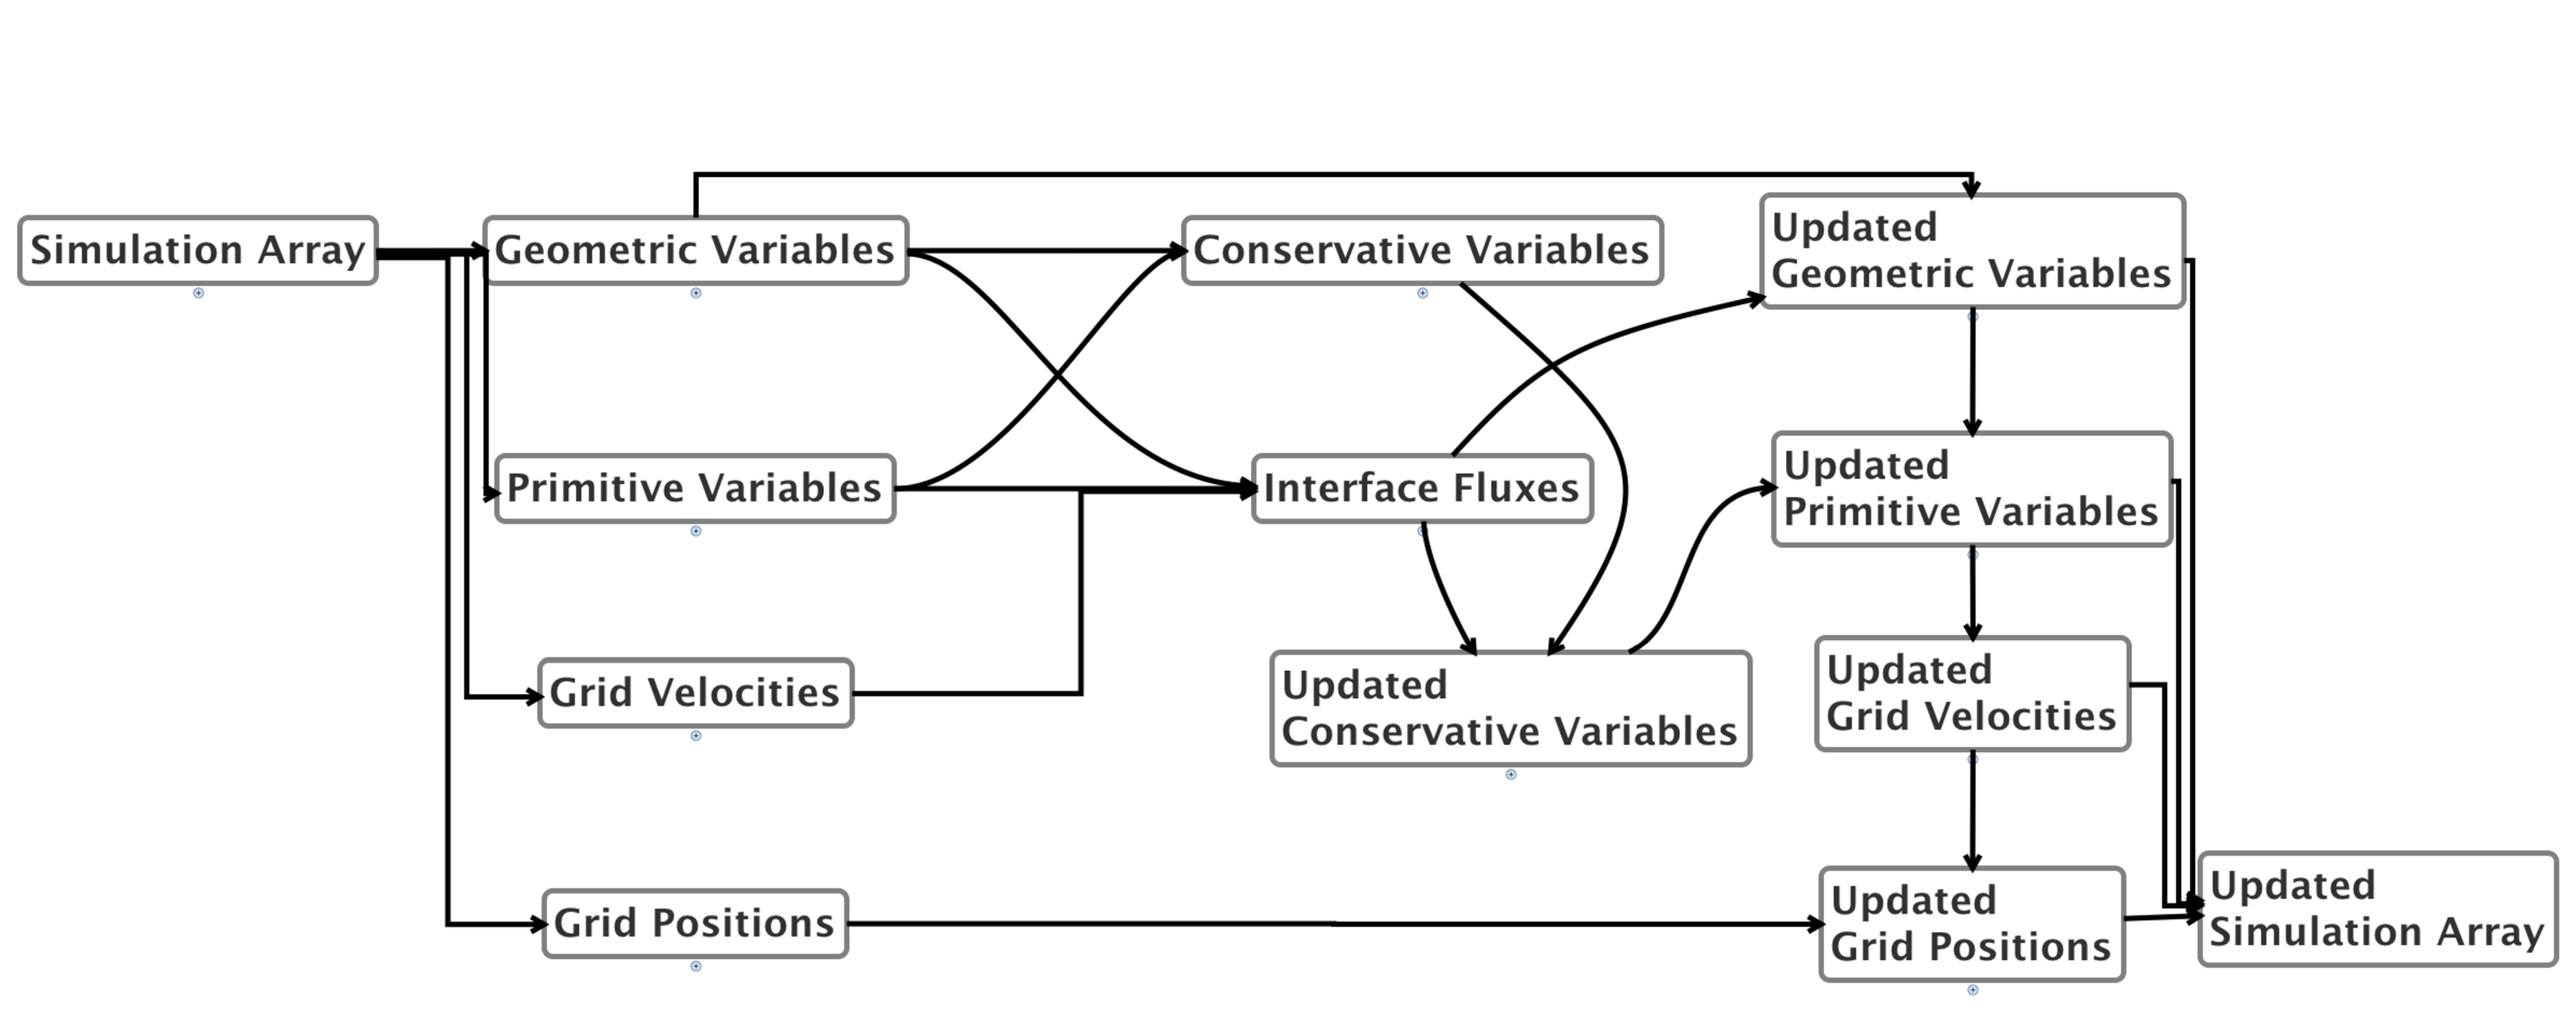
\includegraphics[width=\textwidth]{SimulationFlow.pdf}
\caption[A Diagram of Information Flow in a Unified
CoordinatesProgram]{A diagram of information flow in a unified coordinates program}
\label{fig:simulationflow}
\end{figure}

By artificially decoupling the equations that govern the evolution of the flow from those that govern the metric, the conservation equations (Eq.~\ref{eq:conservation}) reduce to the Euler equations in arbitrary curvilinear coordinates, together with separate, very simple evolution equations for the metric coefficients, and an equation for computing $h$. 

It is also possible to solve the Riemann problem exactly for the one-dimensional transformed equations by decoupling only the equation for $h$ and making additional approximations\cite{hui01}, but the end resulting algorithm is identical in either case.

\subsubsection{MUSCL Refinement}

As the Godunov scheme is only first-order accurate in time, a
flux-limiting, linear, MUSCL interpolation is used to improve the
accuracy to second-order.\cite{toro99} The specific
implementation given by Hui \cite{hui99} is given as:

\begin{equation}
\label{eq:MUSCL}
\begin{array}{c}
f_r=f_{i+1,j}-0.5\left(f_{i+2,j}-f_{i+1,j}\right)\phi\left(r^+\right)\bigskip\\
r^+=\frac{\left(f_{i+1,j}-f_{i,j}\right)}{\left(f_{i+2,j}-f_{i+1,j}\right)}\bigskip\\
f_l=f_{i,j}+0.5\left(f_{i,j}-f_{i-1,j}\right)\phi\left(r^-\right)\bigskip\\
r^-=\frac{\left(f_{i+1,j}-f_{i,j}\right)}{\left(f_{i,j}-f_{i-1,j}\right)}\bigskip\\
\phi\left(r\right)={\rm max}\left(0,{\rm min}\left(1,r\right)\right)
\end{array}
\end{equation}


% \subsubsection{Grid Control}
% Hui recommends that, for flows in which the coefficients $\alpha$ and $\beta$ change sign, the solution of Eq.~\ref{eq:h} be solved by iteration. This has been implemented in the simplest way possible in this work, using a first-order successive over-relaxation scheme. If the coefficients do not change sign, it can also be done using the method of characteristics or variational iteration.

\subsubsection{Boundary Conditions}

Boundary conditions are implemented through the use of ghost cells as
seen in Fig.~\ref{fig:grid}, which are then solved within the Godunov
framework just as any other cell. The flow state within the ghost
cells is chosen according to Table 1.
\begin{figure}[htbp]
   \centering
   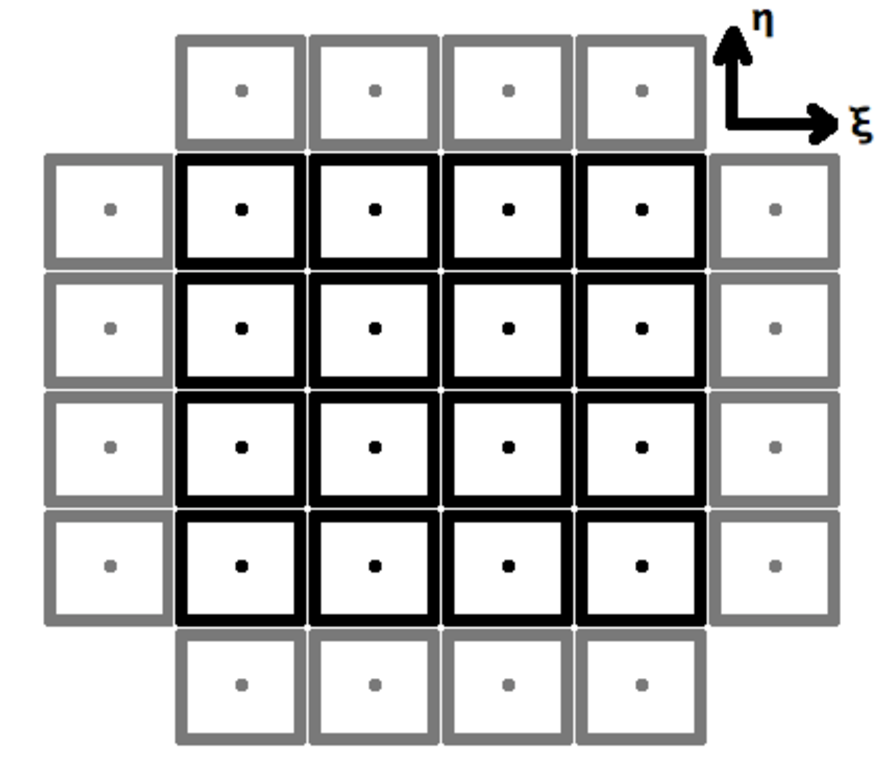
\includegraphics[width=.6\textwidth]{cell_centered_grid_with_ghost_points.pdf} 
   \caption[A Diagram of Computational $\xi$-$\eta$ Space]{Diagram of computational $\xi$-$\eta$ space. Ghost cells are shown in gray.}
   \label{fig:grid}
%   \vspace{-.25in}
\end{figure}

\begin{centering}
\begin{table}
\label{tab:boundary_conditions}
\caption{Application of boundary conditions}
\begin{tabular}{|c|p{.95in}|p{2.75in}|}
\hline
{\bf Boundary Type} & {\bf Specified Quantities} & {\bf How Enforced }\\
\hline
Supersonic Inflow  & All  & Entire flow state is directly specified \\
\hline
Supersonic Outflow & None      & Flow state is copied from simulation interior\\
\hline
Slip (Inviscid Walls)        & Flow Angle  & Flow state is copied from simulation interior. Velocity and metric are reflected across wall angle.\\
\hline
Constant Pressure  & Pressure    & Flow state is copied from simulation interior. Pressure is specified.\\
\hline
\end{tabular}
\end{table}
\end{centering}

The first-order Godunov method requires only the knowledge of directly adjacent cells. For the application of the second-order MUSCL update however, it is necessary to have knowledge of flow states two cells away in each direction. For cell interfaces that correspond to simulation boundaries, the MUSCL update is neglected. This has no effect on the application of boundary conditions, which are satisfied at the interface regardless. For interior cells, the boundary condition is applied normally whenever the MUSCL update reaches beyond the boundary.

% \paragraph{Supersonic Inflow/Outflow}
% \paragraph{Subsonic Inflow/Outflow}
% \paragraph{Streamline Conditions}
% \subparagraph{Reflective Wall Boundary}
% \subparagraph{Constant Pressure Boundary}
\subparagraph{Grid Communication Boundary}
In order to introduce flows consisting of more than a single
streamtube, such as would be required for a two-dimensional airfoil,
it is necessary to implement some form of communication between
separate grids. One way to do this is via boundary conditions applied
at grid interfaces. This will be done with ghost cells as well.
\subsubsection{Coordinate Advancement}

At the end of each time step, the $x$ and $y$ locations of each node must be updated. Trapezoidal integration is both simple and effective, maintaining second-order accuracy at low computational cost. 

\begin{align}
x_{i,j}^{n+1}=&x_{i,j}^{n}+\frac{1}{2}\left(U^n_{i,j}+U^{n+1}_{i,j}\right)\Delta\tau\\
y_{i,j}^{n+1}=&y_{i,j}^{n}+\frac{1}{2}\left(V^n_{i,j}+V^{n+1}_{i,j}\right)\Delta\tau
z_{i,j}^{n+1}=&z_{i,j}^{n}+\frac{1}{2}\left(W^n_{i,j}+W^{n+1}_{i,j}\right)\Delta\tau
\end{align}
\nomenclature[]{$n$}{Time-step index}

\subsection{Steady Riemann Problem}
In order to perform a reliable verification, it is important to stress
the solver. The Riemann problem given by Hui\cite{hui99}, with its three distinct 
nonlinear waves, provides such a stress. It is given by the upstream
boundary condition (See Fig.~\ref{fig:steadyriemann}): 

\begin{equation}
\left(p,\rho,Ma,\theta\right)=\left\{
\begin{array}{lr}
\left(0.25,0.5,7,0\right) & :y>0\\
\left(1,1,2.4,0\right) & :y<0
\end{array}
\right.
\end{equation}
\noindent where $Ma$ is the Mach number and $\theta$ is the flow angle given by
$u=\left|\vec{u}\right|\cos{\theta}$,
$v=\left|\vec{u}\right|\sin{\theta}$.
\nomenclature[]{$Ma$}{Mach number}
\nomenclature[]{$\theta$}{Flow angle}

%%Insert Riemann problem figure here 
\begin{figure}[htbp]
\centering
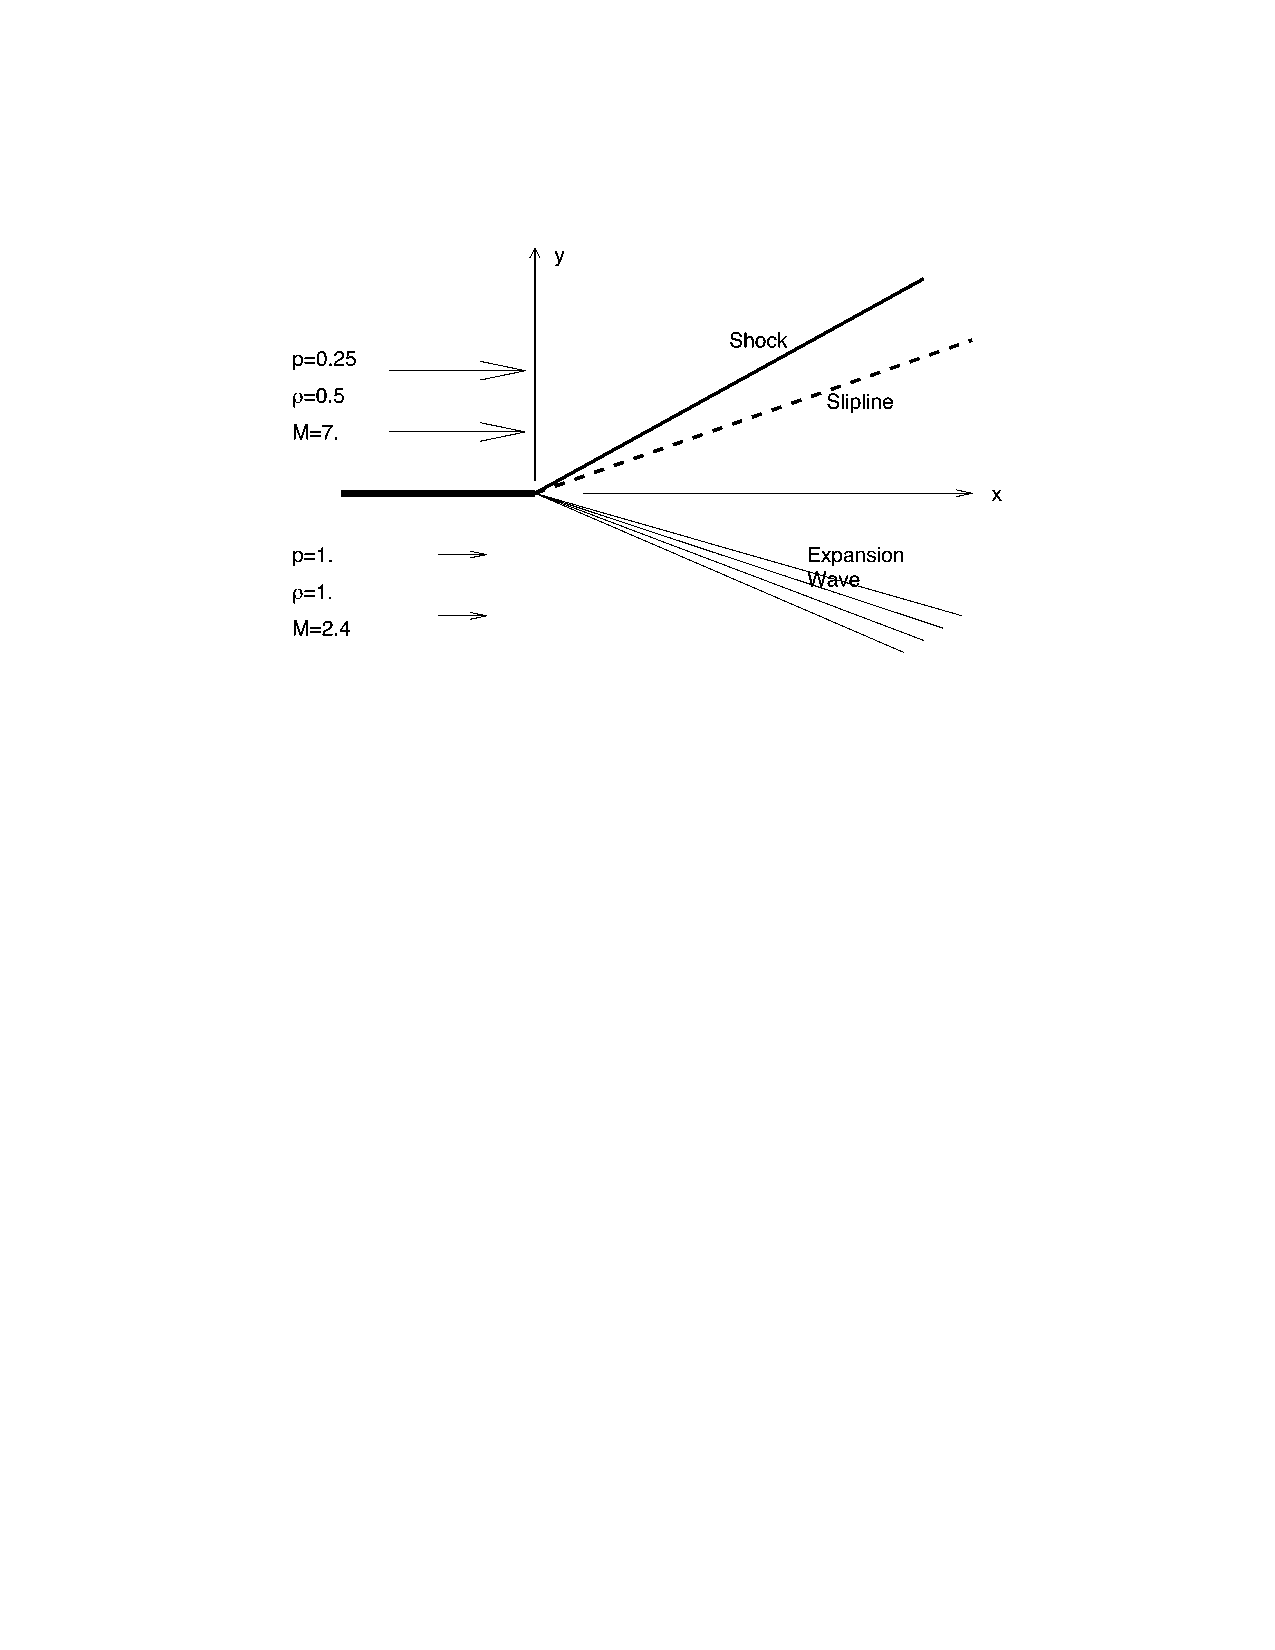
\includegraphics[width=\textwidth]{steadyriemann.pdf}
\caption[A Diagram of the Steady Riemann Problem]{A diagram of the steady Riemann problem, as given by
  Hui\cite{hui99}}
\label{fig:steadyriemann}
\end{figure}

%As previously mentioned, 
The solution to this problem contains a shock, an expansion wave, and a slip line, which come together at a singularity at the origin.
Figs.~\ref{fig:riemann_similarity_0} and \ref{fig:riemann_similarity_9} demonstrate the greatly improved resolution of the slip line when using unified coordinates as compared to the traditional Eulerian coordinate system, and reveal the sacrifice of accuracy near the expansion fan. 

\begin{figure}[htbp]
   \centering
      \begin{subfigmatrix}{2}
        \subfigure[$h = 0$ (Eulerian)]{\label{fig:riemann_similarity_0}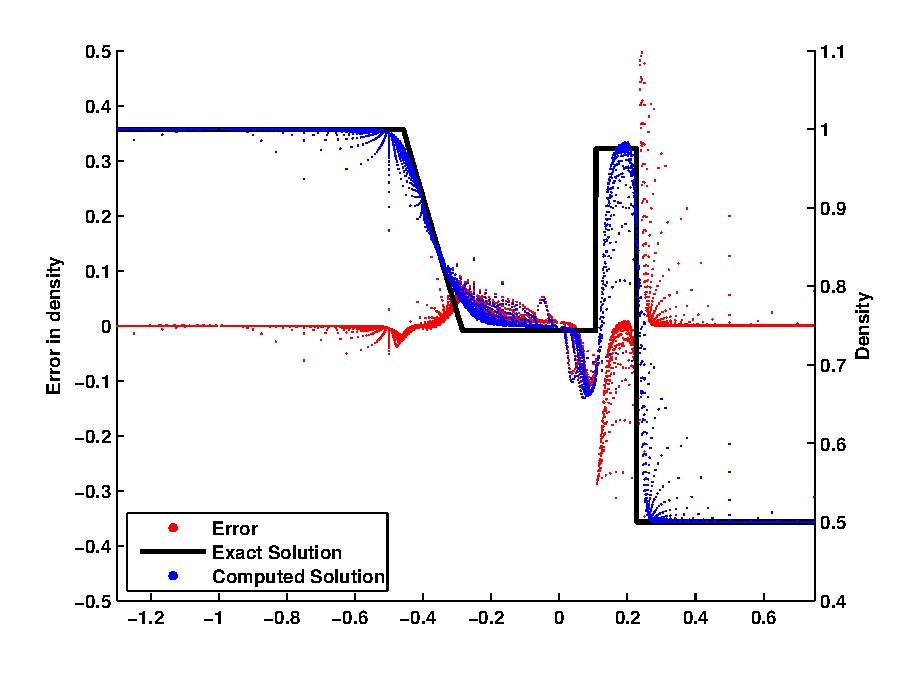
\includegraphics[width=.45\textwidth]{density_error_0.pdf}}
        \subfigure[$h = 0.999$ (Unified)]{\label{fig:riemann_similarity_9}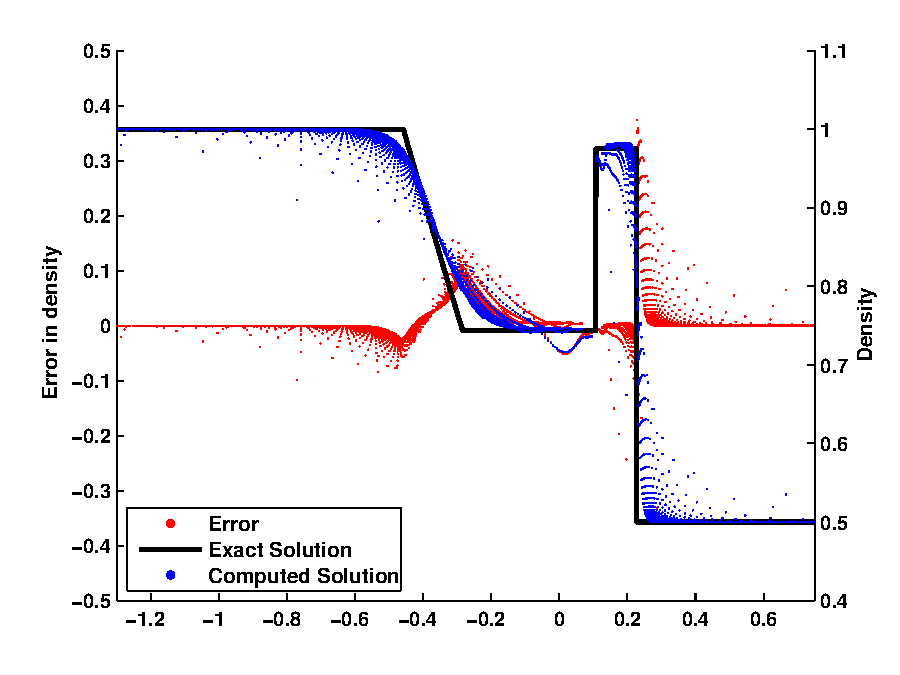
\includegraphics[width=.45\textwidth]{density_error_9.pdf}}
      \end{subfigmatrix}
   \caption[The Similarity Solution of the Riemann Problem]{The similarity solution of the Riemann problem and the corresponding error in the numerical solution, computed throughout the simulation region.}
   \label{fig:riemann_similarity}
\end{figure}

%\begin{figure}[htbp]
%   \centering
   
%   \caption{The similarity solution of the Riemann problem and the corresponding error in the numerical solution, for a Eulerian-style mesh.}
%   \label{fig:riemann_similarity0}
%\end{figure}

\begin{figure}[htbp]%{r}{.6\textwidth}
   \centering
%   \vspace{-.25in}
   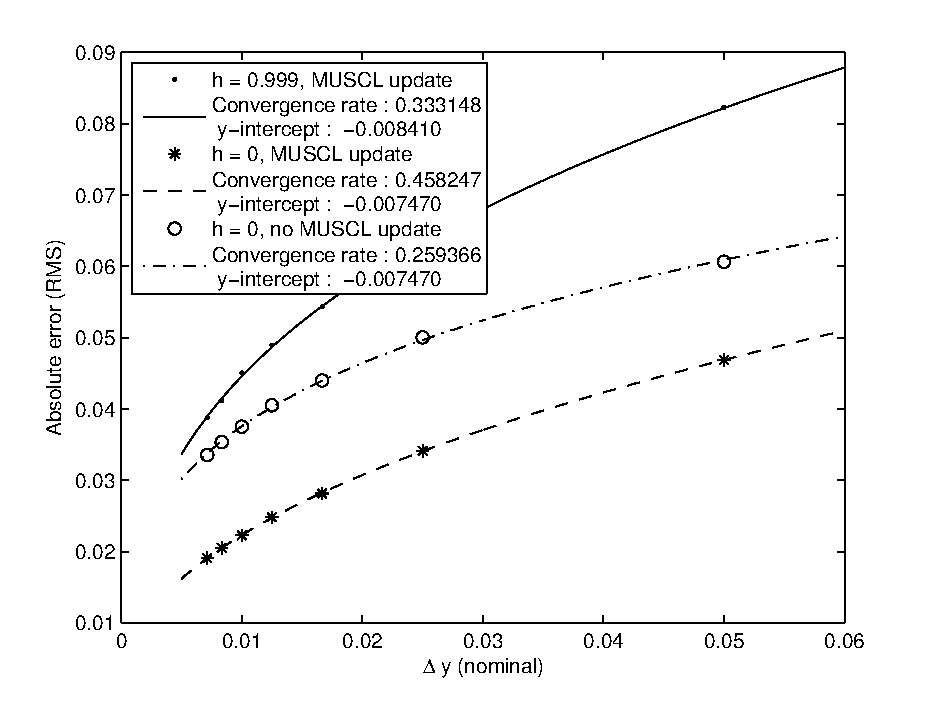
\includegraphics[width=\textwidth]{Riemann_convergence.pdf} 
   \caption[Convergence of Riemann problem]{Root-mean-squared error for the Riemann problem, with order of convergence $n$.}
   \label{fig:riemann_convergence}
%   \vspace{in}
\end{figure}

Fig. \ref{fig:riemann_convergence} quantifies these findings. The solution is shown to converge in three different test configurations, albeit with lower convergence rates than were expected.
However, some recent results have been obtained for other verification
problems, and the end behavior is not yet understood. Further work is
required in this area. 

% It is known that monotone finite difference methods such as the plain
% Godunov method, are 1/2-order accurate overall\cite{sabac97}. Hui's
% unified coordinate scheme is formally second-order based on the minmod limiter, and therefore should be at least 5/8-order accurate\cite{popov05}. In the results shown here, the observed convergence rates are markedly lower.
% There are several possible explanations for this behavior: 
% \begin{itemize}
% \item When the computational mesh is moving, the singularity at the upstream boundary is imperfectly resolved, and its apparent location may vary as cells move by. 
% \item Boundary conditions in general are applied using only first-order accurate methods. 
% \item The error of the time-step-eulerian approximation is unknown. 
% \item The Strang dimensional splitting approximation used here is only first-order. 
% \end{itemize}


% \subsubsection{Problem Description}
% \paragraph{Boundary Types Exercised}
% \subsubsection{Analytical Solution}
% \subsubsection{Numerical Solution}
% \subsubsection{Grid Convergence Analysis}
\subsection{The Oblique Shock}

In order to further verify the unified coordinates method, we run a test problem for an oblique shock wave. The upstream condition is given by 
\begin{equation}
\left(p,\rho,M,\theta\right)=\left(1,1,1.8,0\right)
\end{equation}
\noindent and the wall angle that induces the shock is chosen to give
a downstream flow angle of $45^o$. The grid was generated
automatically, with a value of $h = 0.999$. A preliminary grid
convergence study was performed, and the results are shown in
Fig.~\ref{fig:shock_convergence}.

\begin{figure}[htbp]
  \centering
  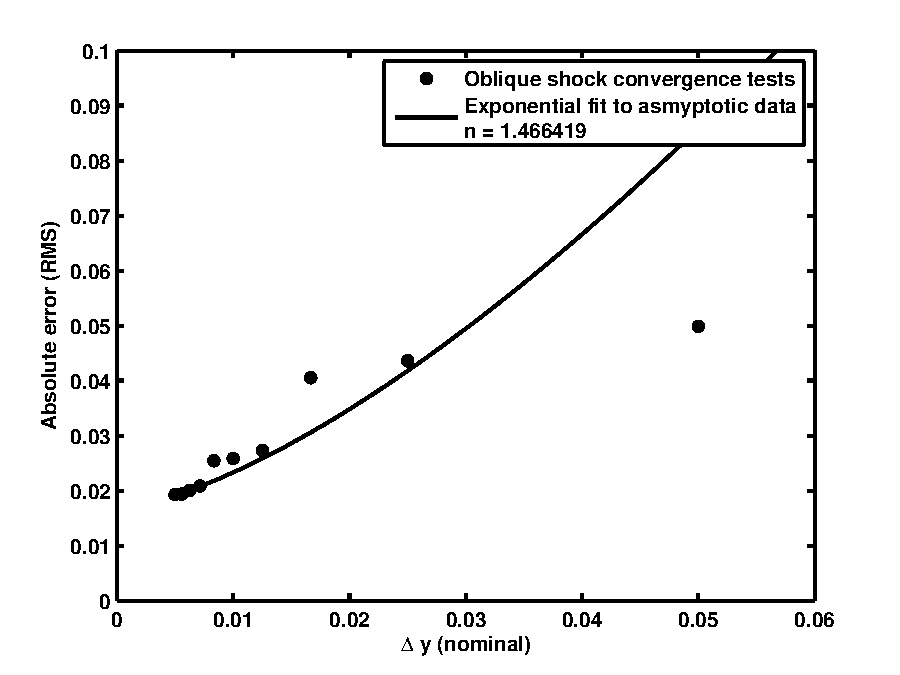
\includegraphics[width=\textwidth]{shock_convergence2.pdf}
  \caption[RMS for the Oblique Shock
  Problem]{Root-mean-squared error for the oblique shock
    problem. Curve is fit to the four highest resolution points
    only.}
  \label{fig:shock_convergence}
\end{figure}

% The root-mean-squared error of the computed solution for the oblique shock closely follows the behavior exhibited by that of the Riemann problem, with one major caveat. As the grid is refined, there is a critical refinement level beyond which oscillations appear in the solution, as seen in Fig. \ref{fig:shock_instabilities}. These oscillations increase the error, though the solution continues to converge.

%\begin{wrapfigure}{l}{.4\textwidth}
%   \centering
%   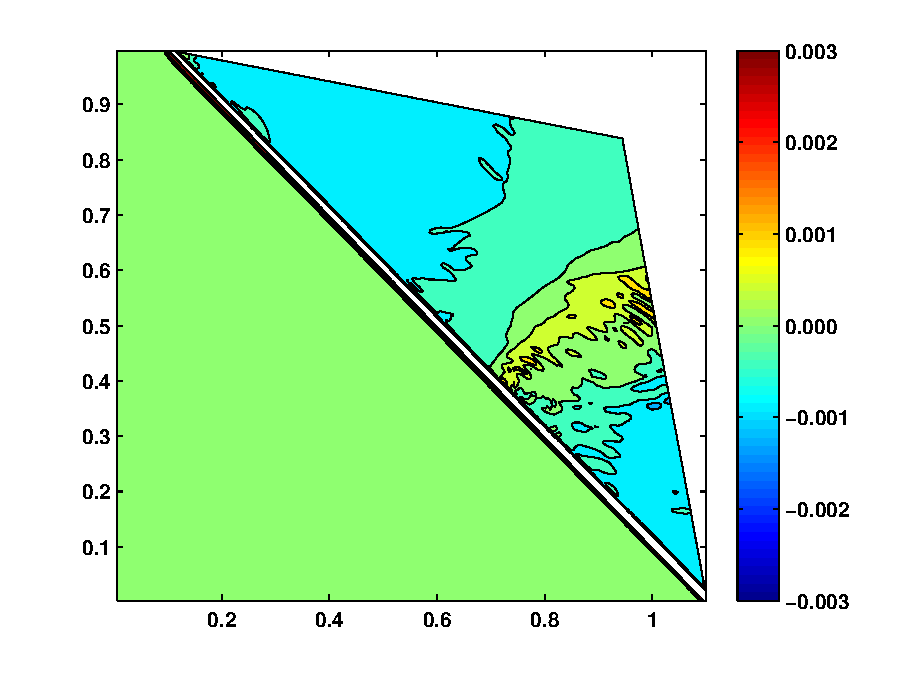
\includegraphics[width=.4\textwidth]{shock_instabilities.pdf}
%   \caption{A plot of normalized error in pressure, highlighting the oscillations which propagate downstream from the oblique shock.}
%   \label{fig:shock_instabilities}
%\end{wrapfigure}
\subsection{Prandtl-Meyer Expansion}
\subsubsection{The Expansion Fan and ``Grid Separation''}

\begin{figure}[htbp]%{r}{.4\textwidth}
   \centering
   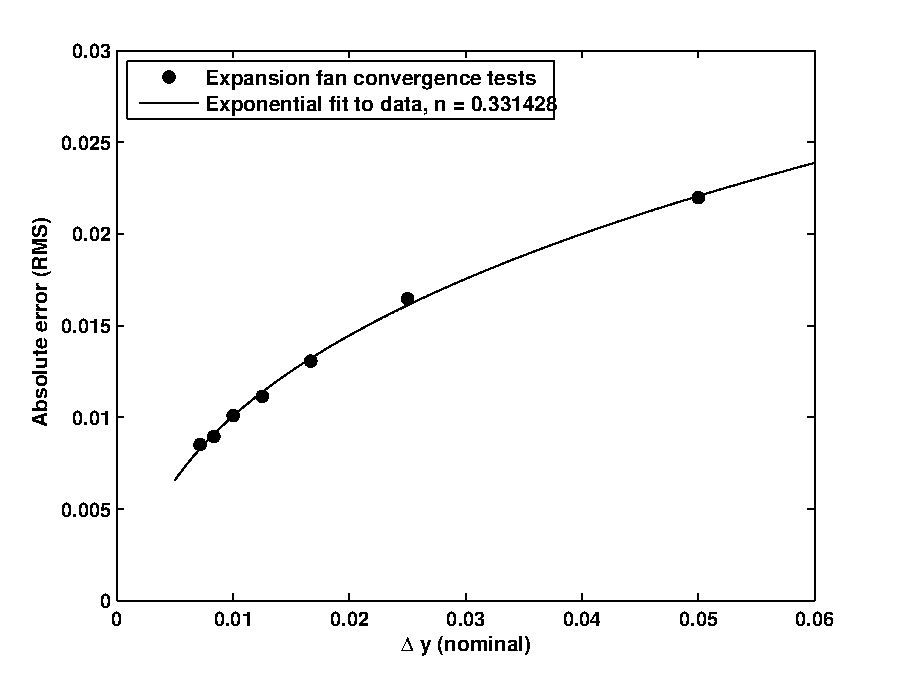
\includegraphics[width=\textwidth]{fan_convergence.pdf} 
   \caption[RMS error for Prandtl-Meyer expansion]{Root-mean-squared error for the Prandtl-Meyer expansion, with order of convergence $n$.}
   \label{fig:expansion_convergence}
%\vspace{-1.in}
\end{figure}

A final verification test was run for a Prandtl-Meyer expansion
corner. Convergence was again demonstrated (see
Fig. \ref{fig:expansion_convergence}), but the expansion corner
reveals an important limitation of the current method. 
In the presence of a strong expansion wave, the decreased grid resolution can cause the computational nodes to pull away from the wall, as can be seen in Fig.~\ref{fig:expansion_separation}. Thus, although the streamlines eventually do align with the wall as expected, the dramatic loss of resolution near the wall may seriously affect any further downstream results.
%As can be seen in Fig. \ref{fig:expansion_separation}, the computational nodes have a tendency to pull away from the wall as the expansion angle increases. The effect of this is to reduce grid resolution at the wall, and the appearance is very similar to that of boundary layer separation. 

\begin{figure}[htbp] %  figure placement: here, top, bottom, or page
   \centering
   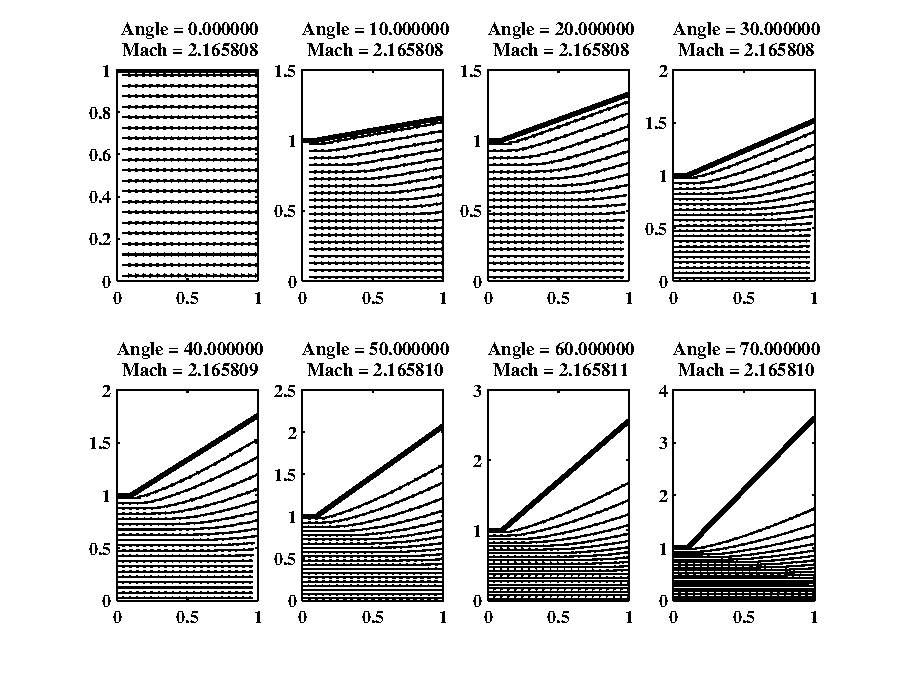
\includegraphics[width=\textwidth]{Expansion.pdf} 
   \caption[Computed Streamlines for Edxpansion at Increasing Angles]{Computed streamlines for expansion at increasing angles. Angles are given in degrees.}
   \label{fig:expansion_separation}

\end{figure}

% \subsubsection{Problem Description}
% \paragraph{Boundary Types Exercised}
% \subsubsection{Analytical Solution}
% \subsubsection{Numerical Solution}
% \subsubsection{Grid Separation}
\subsection{Diamond Shock Train}
The unified coordinate system is especially useful for problems where the physical boundaries themselves are unknown, such as pressure boundary conditions. Consider the nozzle plume flows in Fig. \ref{fig:nozzle_flow}, which were generated with constant pressure boundary conditions with no more difficulty than a parallel-wall channel. The mesh itself simply flows to fill 
the streamtube defined by the nozzle, freeing the user from defining
exactly where boundaries lie. In contrast, using traditional methods, an estimate would have to be made of the maximum diameter of the nozzle streamtube, and the simulation sized to fit around that maximum diameter.

\begin{figure}[htbp]
   \centering
%   \vspace{-.5in}
   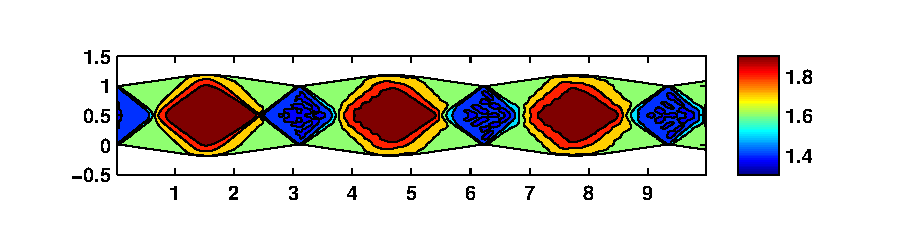
\includegraphics[width=\textwidth]{diamond_shock_train.pdf}
   \caption[Computed Mach Number for Diamond Shock Train]{Computed Mach number for an under-expanded nozzle flow, showing the diamond-shock train}
   \label{fig:nozzle_flow}
\end{figure}

% \subsubsection{Problem Description}
% \paragraph{Boundary Types Exercised}
% \subsubsection{Numerical Solution}
% \paragraph{Stream Boundary Identification}

\subsection{A Transonic Duct Flow}

Finally, we use the unified coordinates method to model flow through a
convergent duct. This problem is identical to the one given by
Hui\cite{hui99}, and is characterized by the formation of a mach stem
and the resulting transonic flow
(Fig.~\ref{fig:shock_train_channel_flow}). The mesh again flows
through the duct, conforming to solid walls without need for user
specification of the mesh. 

\begin{figure}[htbp] %  figure placement: here, top, bottom, or page
   \centering
   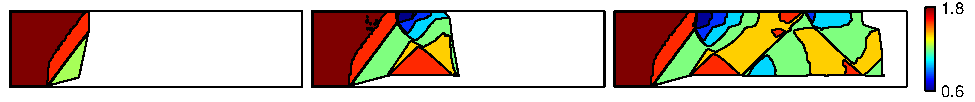
\includegraphics[width=6in]{Channel_flow_filmstrip_image_mach.pdf} 
   \caption[Time-Lapse Images of Transonic Duct Flow]{Computed Mach
     number for transonic duct flow at various times, showing the
     manner in which nodes flow to fill boundaries.}
   \label{fig:shock_train_channel_flow}
\end{figure}

\begin{figure}[htbp]
   \centering
   \begin{subfigmatrix}{2}
      \subfigure[$h=0$, nominal grid size: $72 \times 20$]{
   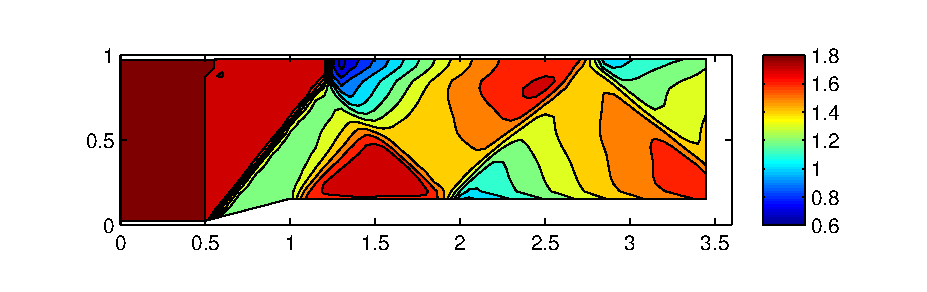
\includegraphics[width=.45\textwidth]{shock_train_contourh00p4.pdf}
   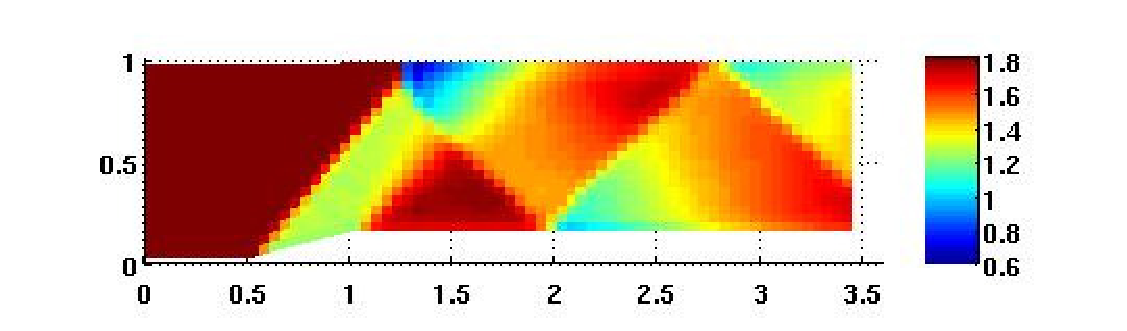
\includegraphics[width=.45\textwidth]{shock_train_surfh00p4.pdf}}
      \subfigure[$h=0.25$, nominal grid size: $72 \times 20$]{
   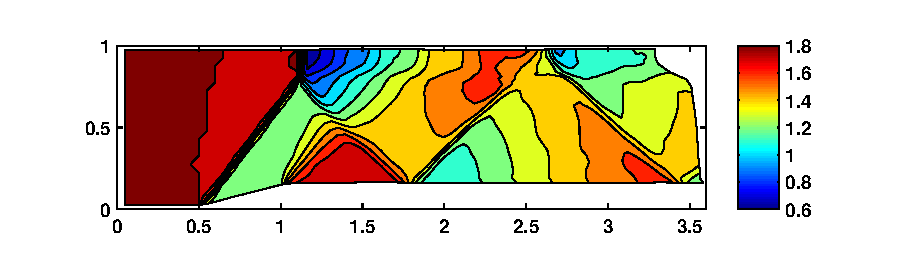
\includegraphics[width=.45\textwidth]{shock_train_contourh250p4.pdf}
   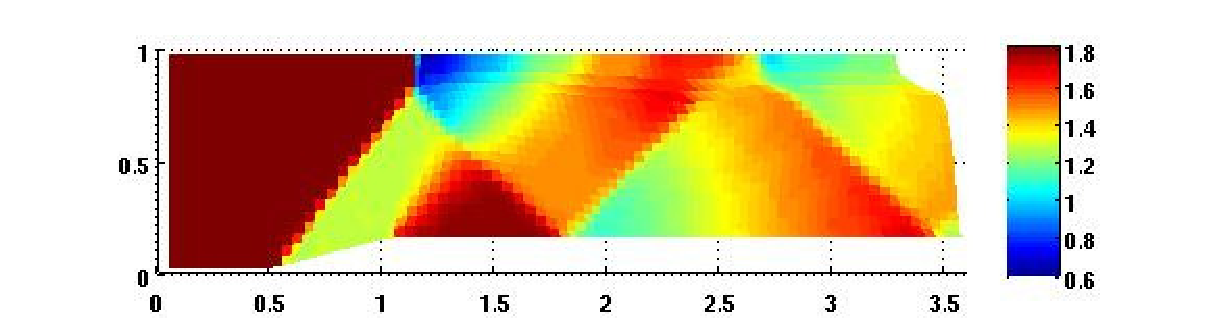
\includegraphics[width=.45\textwidth]{shock_train_surfh250p4.pdf}}
      \subfigure[$h=0$, nominal grid size: $360 \times 100$]{
   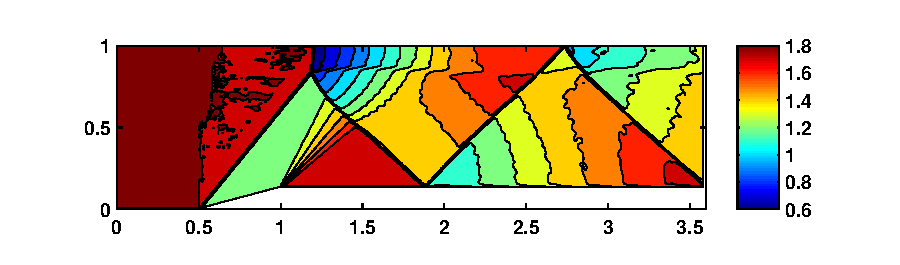
\includegraphics[width=.45\textwidth]{shock_train_contourh02p0.pdf}
   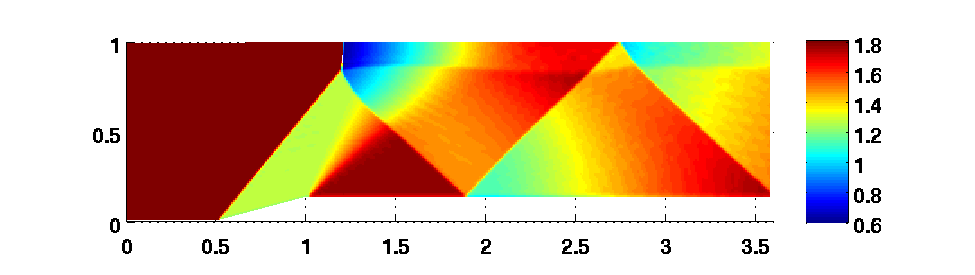
\includegraphics[width=.45\textwidth]{shock_train_surfh02p0.pdf}}
   \end{subfigmatrix}
   \caption[Accuracy Comparison Between Moving and Stationary
   grids]{Qualitative accuracy comparison between Unified ($h=0.25$)
     (b) and Eulerian ($h=0$) (a,c) simulations for a transonic duct
     flow. Notice the improved resolution of the slip line and the
     walls for the unified solution.}
   \label{fig:duct_verification}
\end{figure}
   

%Although the verification done for the Riemann problem was less than encouraging, the duct flow problem tells a different story, at least qualitatively. 
It can be seen in Fig. \ref{fig:duct_verification} that the Eulerian
scheme ($h = 0$) fails to capture the formation of the slip line at
low grid resolutions, and also shows slightly less accurate prediction
of shock locations when compared with a much higher resolution
solution. The unified coordinates  method, on the other hand, does
resolve the slip line, and makes slightly more accurate predictions of
shock locations, at the cost of a less-well-resolved expansion corner.  

\subsection{Basic Boundary-Layer Effects in a Uniform Channel}

Many phenomena in hypersonics are a result of the interaction of the
viscous boundary layer with the inviscid flow. As a result, some
method of accounting for viscous effects is almost a requirement for
hypersonic flows, and
boundary-layer methods provide this at minimal cost. 

A crude, prototypical implementation uses the turbulent, flat-plate,
constant pressure formula given in
Schlichting\cite{schlichtingblayer}: 
\begin{equation}
  \frac{\delta u_\infty}{\nu}=0.14\frac{Re_x}{\log{Re_x}}G(\log Re_x)
\nomenclature{$u_\infty$}{Inviscid core velocity condition for
  boundary-layer}
\nomenclature{$Re_x$}{Reynolds number with respect to $x$}
\nomenclature{$\nu$}{Kinematic viscosity}
\end{equation}
\noindent where $G$ is taken to be the limiting value of $1$.

This serves as a useful proof-of-concept for the method, and will be a
valuable step toward implementation of an actual boundary-layer solver. In
the inviscid simulation, boundary-layer effects are included by
enforcing a solid wall 
condition that aligns with the boundary-layer displacement thickness.

Results from one such proof-of-concept test are shown in
Fig.~\ref{fig:bl_shock_train}. The presence of the boundary layer can
be clearly seen in the curving of the inviscid flow in the otherwise
uniform channel, as well as the formation of the oblique shock train. 

\begin{figure}[htbp]
  \centering
  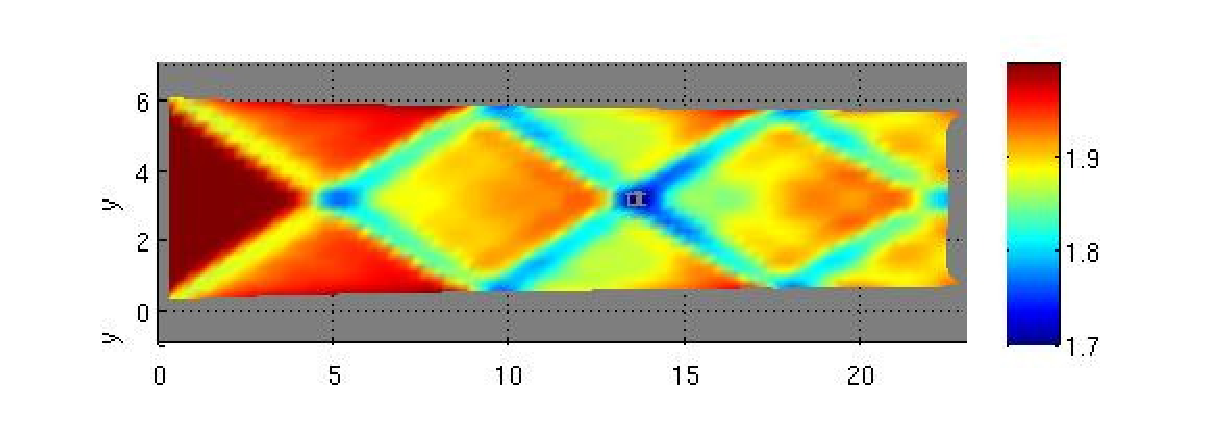
\includegraphics[width=\textwidth]{BL_shock_train2.pdf}
  \caption[Channel Flow With a Turbulent Boundary Layer]{Oblique shock train produced by a turbulent boundary layer in an otherwise uniform channel}
  \label{fig:bl_shock_train}
\end{figure}

\subsection{Model F-14 Inlet}

One of the principal attractions of the unified coordinates method is the potential to represent complex flow geometries in a simple, intuitive way and without grid generation. To better illustrate this feature, a more complex inlet model was chosen, based off of publicly available sketches of the inlet of the now retired USAF F-14. This inlet is approximately two-dimensional and is designed to provide subsonic flow to the engine at freestream Mach number in the range $0<M<2.3$. This is accomplished through the use of internal, variable ramps, as shown in Fig.~\ref{fig:f-14_diagram}.

This is exactly the kind of problem the unified coordinates can excel at. Defining an
approximate flow geometry is simple, and the automatic grid generation
allows for quick solutions at different freestream conditions, and the
correspondingly different inlet geometries. 

An example based on the F-14 inlet is shown in
Fig.~\ref{fig:f-14_flow}, but the results are  
only prototypical. Due to as-yet-unimplemented
features such as multi-stream capability and subsonic outflow
conditions, it is not possible to correctly model spillage, nor is it
possible to achieve subsonic flow in the inlet. Further testing will
be possible once these features have been added.

\begin{figure}[htbp]
   \centering
   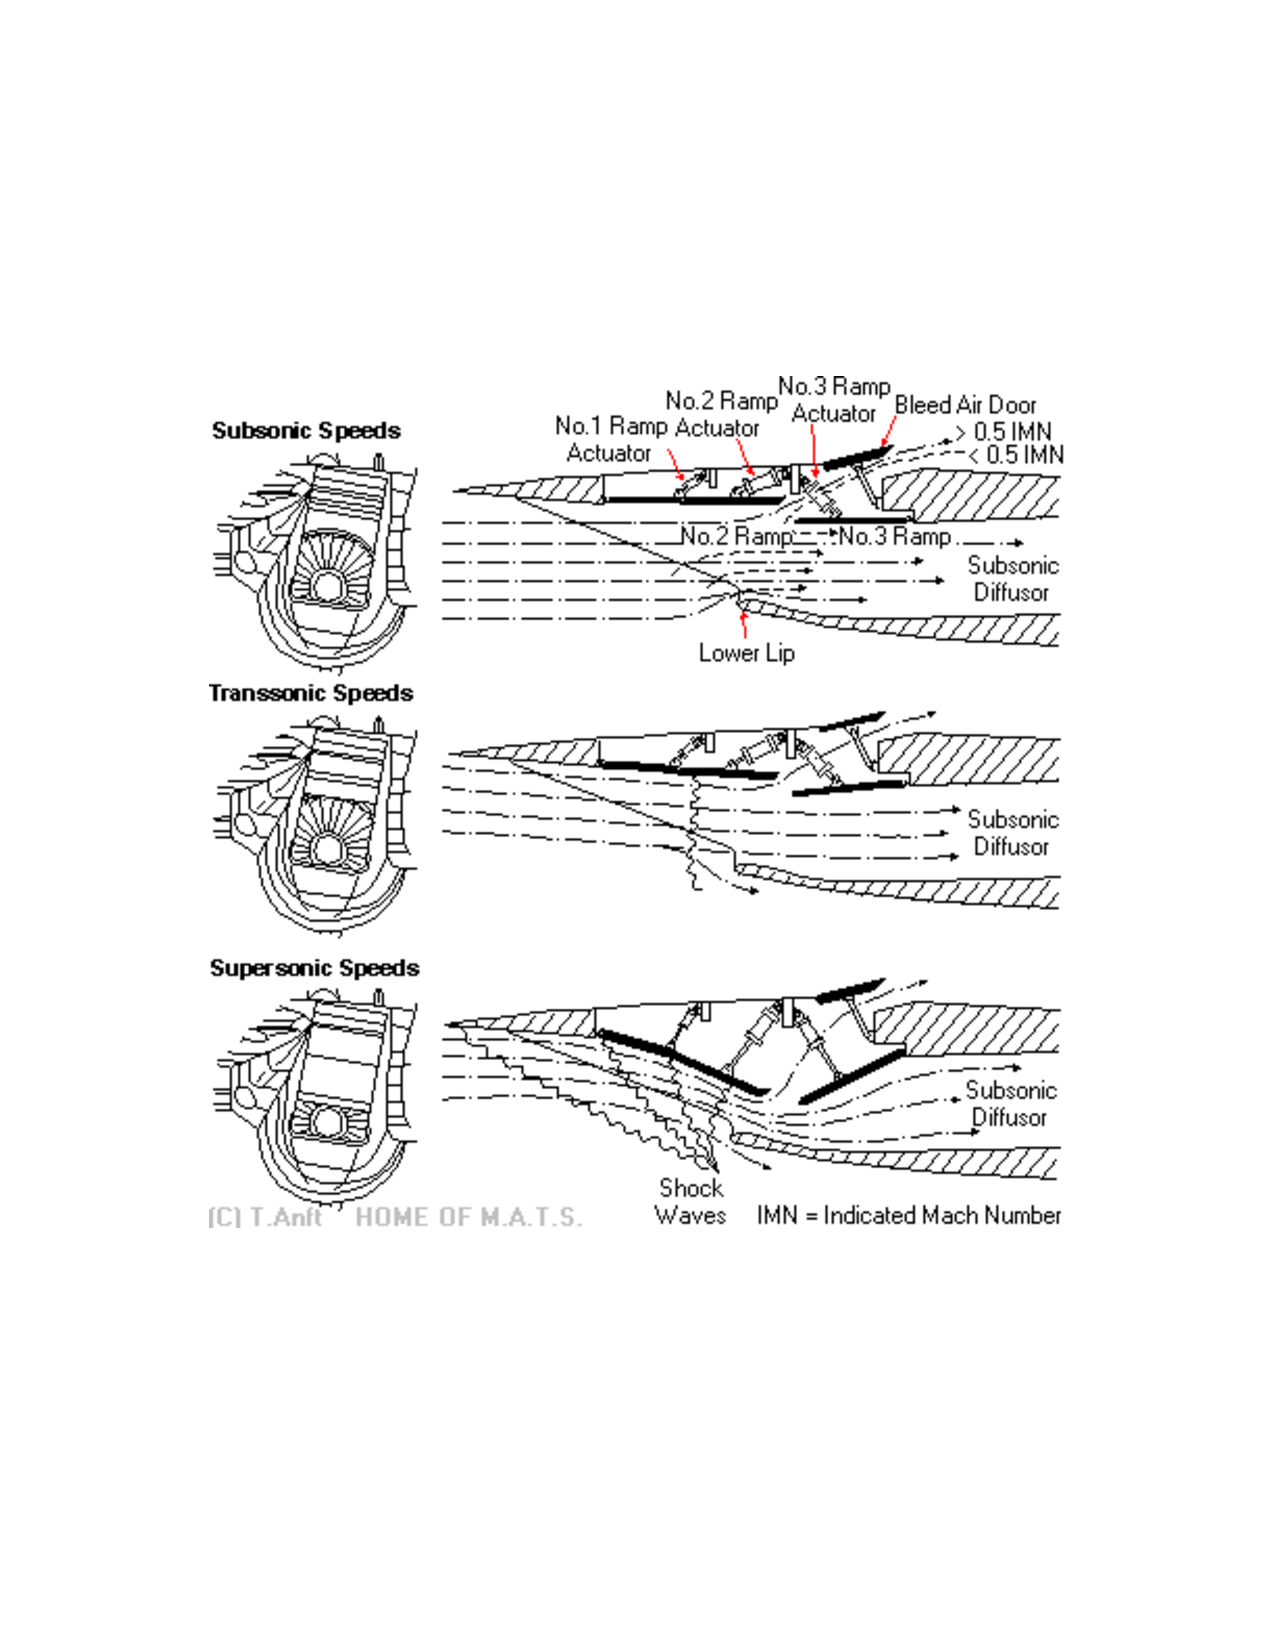
\includegraphics[width=\textwidth]{F_14_inlet_diagram.pdf}
   \vspace{-1.5in}
   \caption[Diagram of USAF F-14 Tomcat]{Diagram of the variable inlet
     geometry of the USAF F-14 Tomcat. Courtesy of: Home of M.A.T.S.,
     Available at http://www.anft.net/f-14/f14-detail-airintake.htm,
     Accessed 25 Nov 2011}
   \label{fig:f-14_diagram}
\end{figure}

% Unfortunately, shock-induced instabilities have plagued this effort. It was impossible to obtain a full steady-state solution, and it was likewise impossible to resolve any subsonic or transonic flows. The full solution of this problem will therefore require further refinement and verification of the solution methodology. A completely supersonic flow, having not quite come to steady-state, is shown in Fig.~\ref{fig:f-14_flow}, and the growing instabilities are visible in the last frame.

\begin{figure}[htbp]
   \centering
   % 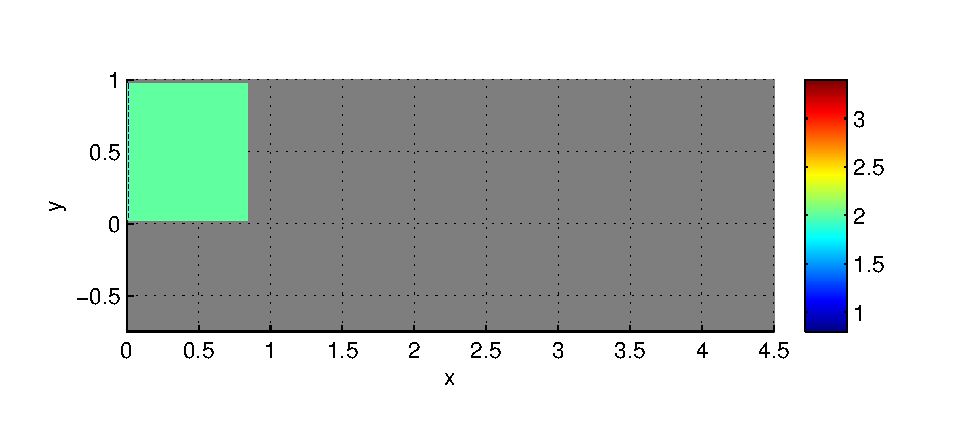
\includegraphics[width=.4\textheight]{F_14_filmstrip_1.pdf}
   % 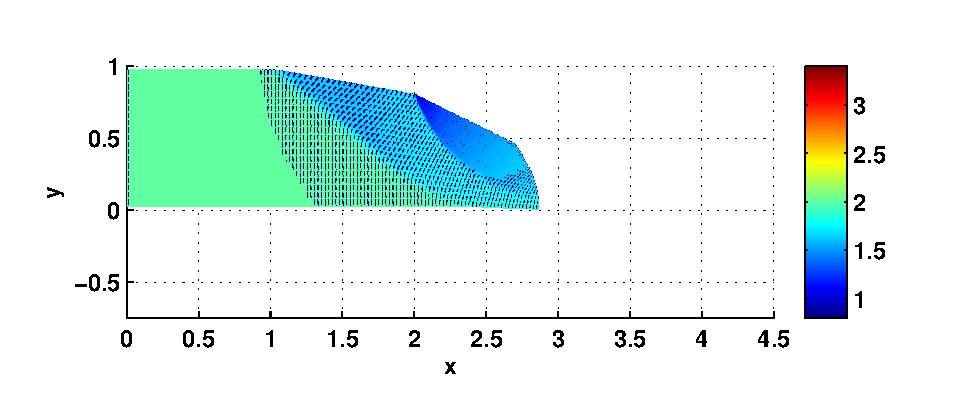
\includegraphics[width=.4\textheight]{F_14_filmstrip_2.pdf}
   % 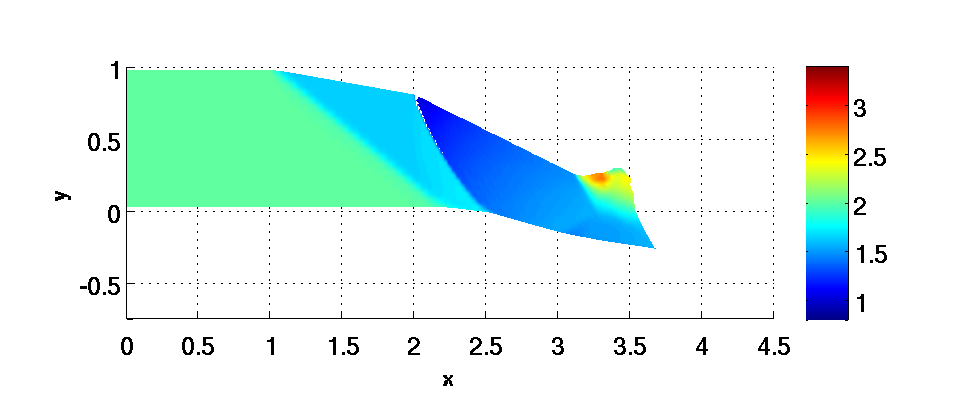
\includegraphics[width=.4\textheight]{F_14_filmstrip_3.pdf}
   % 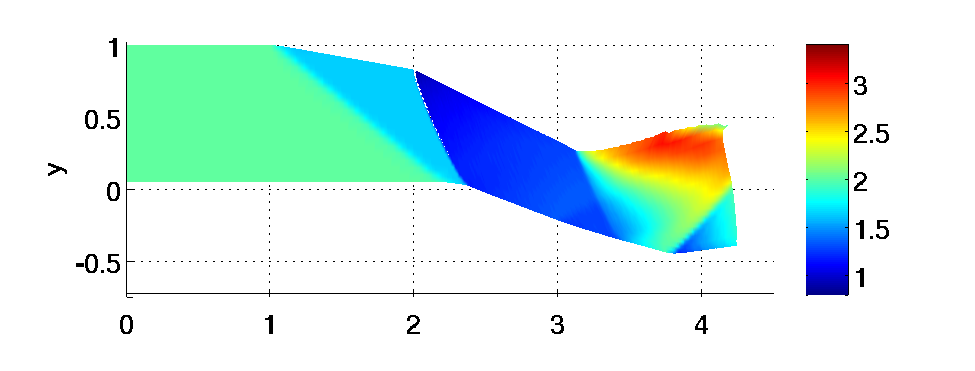
\includegraphics[width=.4\textheight]{F_14_filmstrip_4.pdf}
   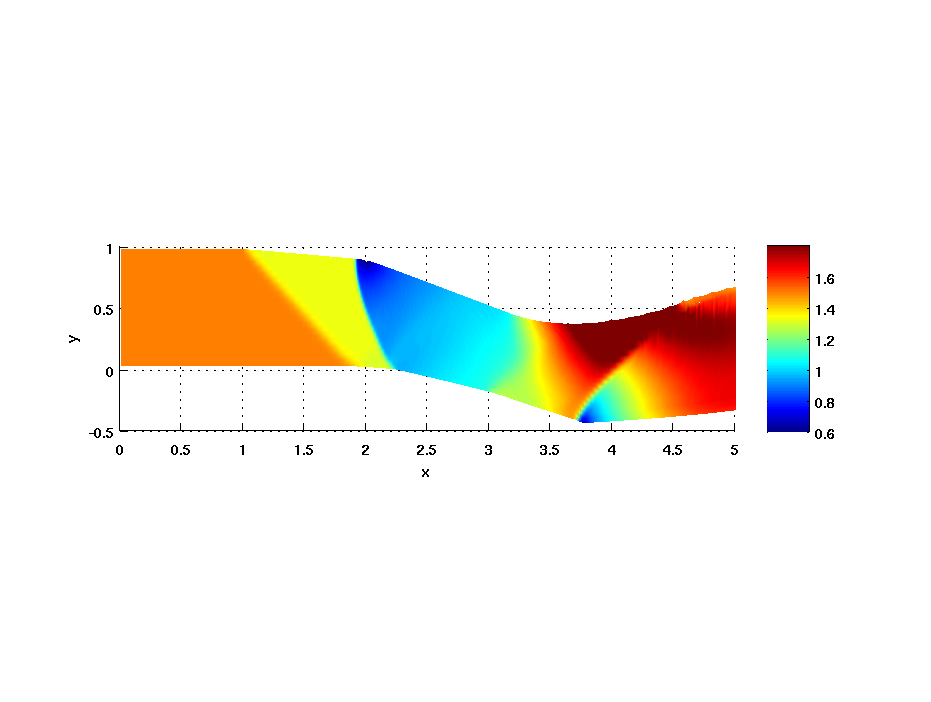
\includegraphics[width=\textwidth]{F_14_filmstrip_5clean.pdf}
   \caption[Mach Number in F-14 Inlet]{Mach number in a geometry modeled after Fig.~\ref{fig:f-14_diagram}.}
   \label{fig:f-14_flow}
\end{figure}


\section{Proposal \& Timeline}
\label{sec:timeline}
\begin{figure}[htbp]
   \centering
   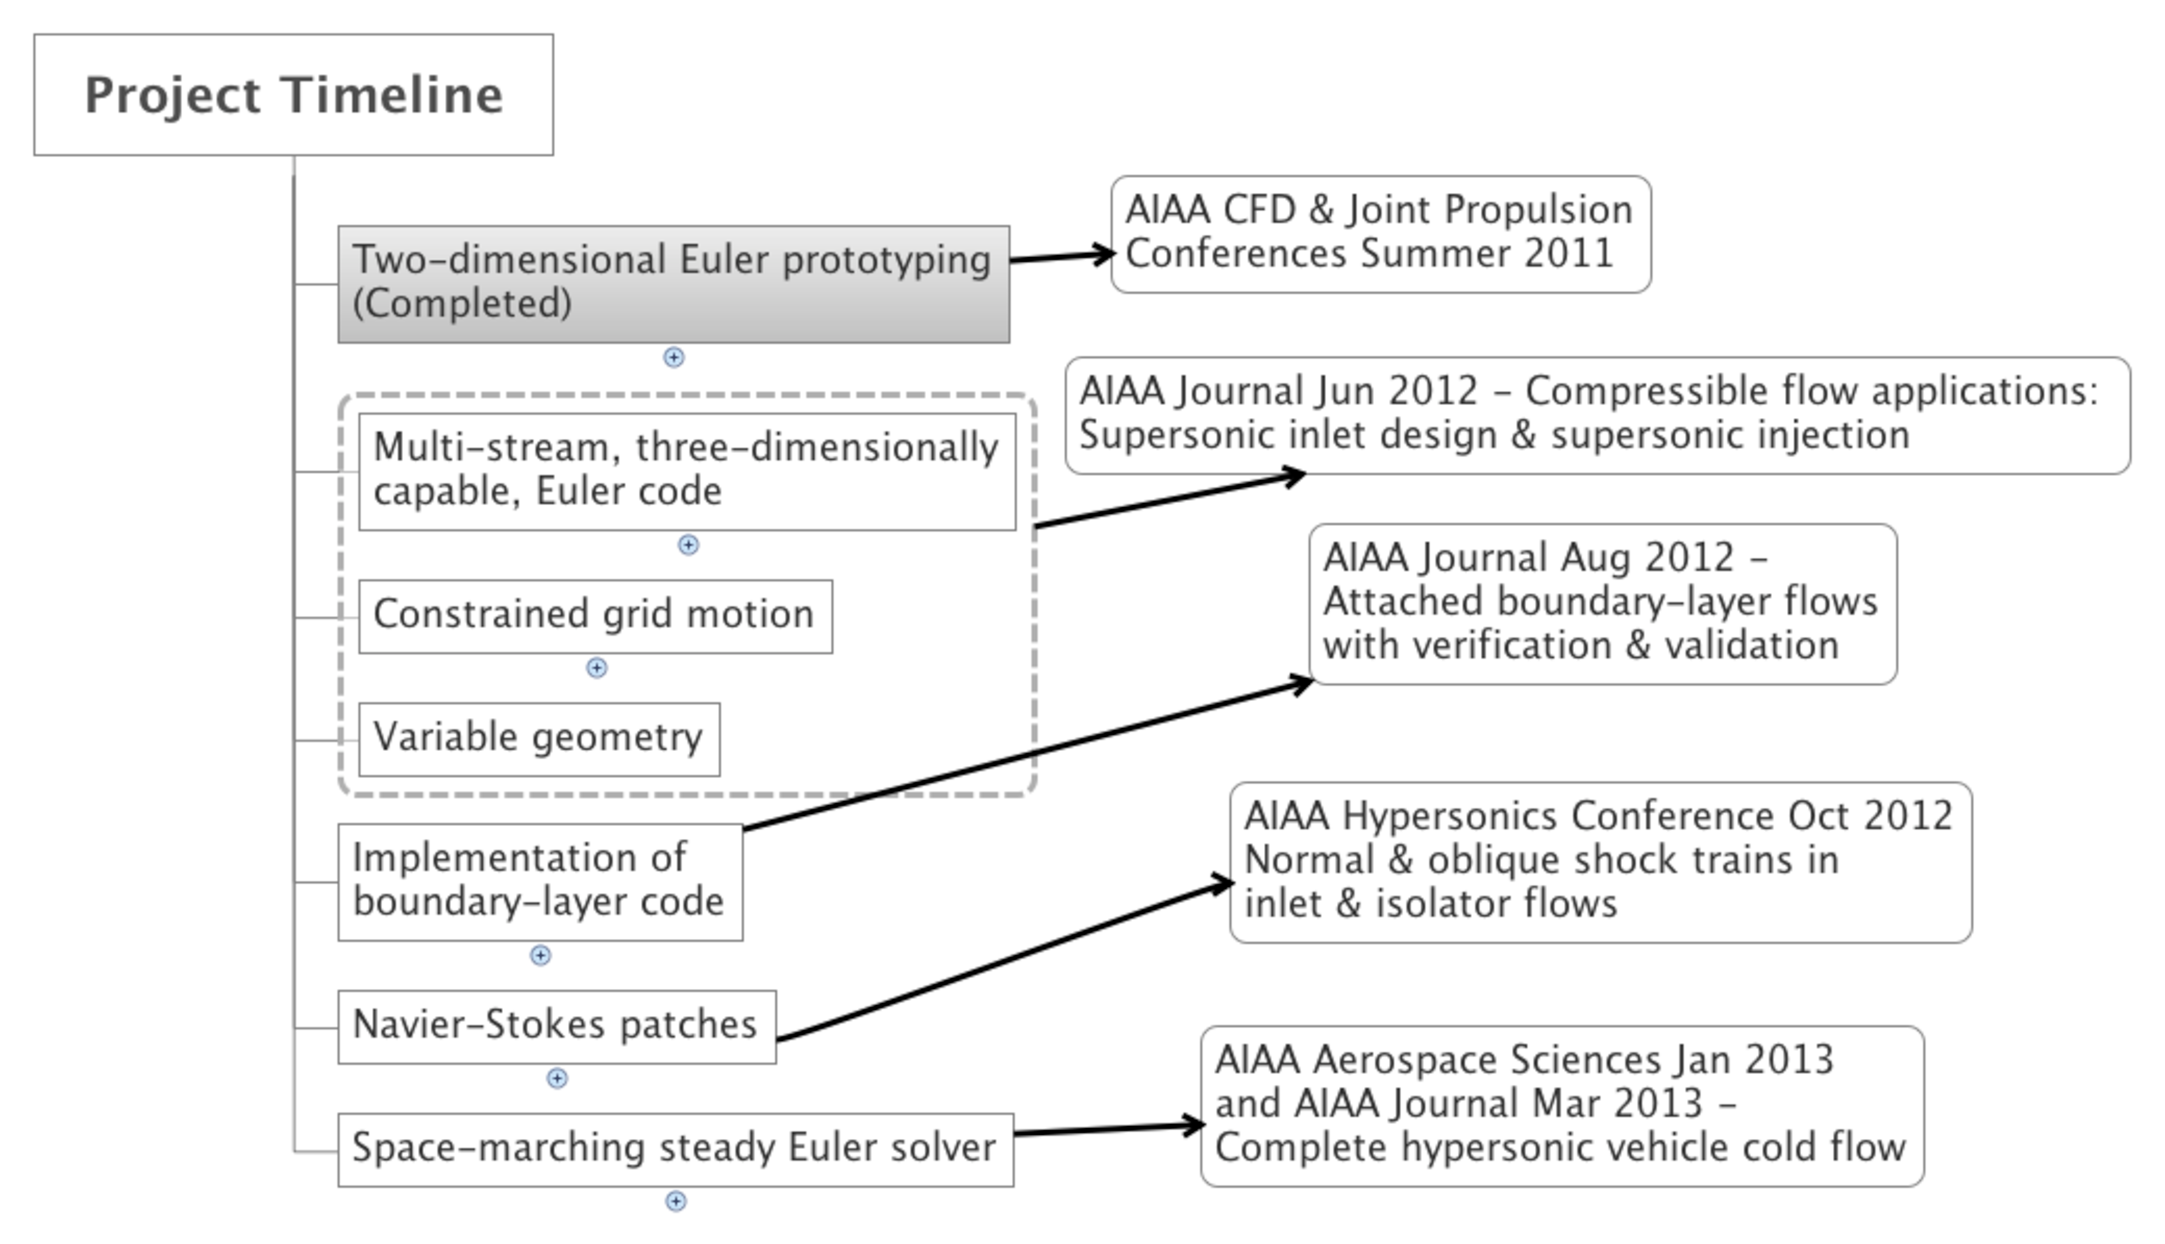
\includegraphics[width=\textwidth]{Timeline.pdf}
  \caption[Proposed Timeline for Dissertation Work and
  Publications]{Proposed timeline for dissertation work \&
    publications} 
   \label{fig:dissertation_timeline}
\end{figure}

Although much has already been done to advance the capabilities of the
unified coordinate system, more remains if it is to become a
successful design tool. The disparate pieces discussed in
Sec.~\ref{sec:background} need to be combined in an intuitive,
automatic way, that minimizes human interaction and keeps
computational costs low. I propose to create this design tool by
combining inviscid, viscous, and boundary-layer solvers within a
wrapping program that handles grid generation, boundary
communication, and solver selection. The wrapper will do this
automatically, without the need for human interaction, and requiring
only the boundary conditions and fluid properties as inputs. A
specific project timeline with expected publications is shown in Fig.~\ref{fig:dissertation_timeline}.

\subsection{Multi-Stream, Three-Dimensionally Capable Inviscid Solver}
Although a working time-marching code is available already for
two-dimensional problems, a new code will be written to include also
additional capability and features, such as extensibility to
multi-stream flows and to three-dimensional flows. Although 3-D brings
with it a host of new problems for which solutions are not yet known,
the basic changes to the equation sets are actually quite
simple. Therefore, the code will be written to handle the
three-dimensional equations, but the methods for handling
three-dimensional boundary
conditions will not be developed.
\subsubsection{Three-Dimensional Flows}
\paragraph{Aside - Why not a fully 3-D code}
Three-dimensional flows are much, much more complex than
two-dimensional flows are, no matter what the solver being
used. Unfortunately, because of the unsteady nature of grid cell
boundary conditions in moving grid systems, it would be difficult to
directly leverage the work that has been done in traditional
CFD to solve these problems, and resolving them would therefore
require a substantial investment of time and effort which could be
better spent proving the concepts in the simpler
two-dimensional case, while still enabling many useful applications.

For methods relying on moving grid systems, the most obvious difficulty is
the way in which complex geometries are handled. The marching grid
technique discussed in Sec.~\ref{sec:spatial_discretization}must automatically
detect downstream flow
boundaries and deal with complex, transient, streamtube bending and
tangling. The dynamic update of boundary conditions is also more
difficult. These issues exist for all complex flows, but the
two-dimensional case is much simpler.
\subsubsection{Multi-Stream Flows}
The work that has been done at the Busemann Advanced Concepts Lab on
moving mesh CFD has thus far included only simple flows composed of a
single streamtube. Since that excludes such classic problems as flow
around airfoils, multi-stream capability is an essential component
for any useful design program.
\paragraph{Separate Grids}
Rather than attempt to work with complex and variable
topology on a single grid, multiple
streams will be handled by multiple separate grids which communicate
with one another through their boundary conditions. For the second-order
MUSCL scheme used here, this mandates the use of a double-layer of
ghost cells between grids.
%, a non-trivial but acceptable cost, provided that the aspect ratio
%of the grid remains near unity. 

% \subparagraph{Grid communication}
\paragraph{Aside - MPI Parallelism}
It is worth noting that a multi-stream approach is directly adaptable
to distributed-memory parallelism. This will greatly simplify the
eventual parallelization of the program.
% \subparagraph{Inter-Stream Parallelism}
% \subparagraph{Intra-Stream Parallelism}
\subsubsection{Goals}
\begin{itemize}
\item Communication between multiple streams of inviscid flow -
  Completed 
  by: Mar, 2012, Paper on variable geometry supersonic inlet submitted
  to AIAA Journal, 30 Apr
\item Sample problems - Supersonic injection, wing cross-section with
  verification and validation, supersonic
  inlet (F-14, Concorde)
\end{itemize}
\subsection{Constraining Grid Motion}
Thus far, the Busemann Lab has not implemented a robust method for
grid distortion control. Doing so is a light project, and will require
the derivation of control equations for jacobian- and
skewness-preserving schemes as well for grid-angle-preserving
schemes. It will also require the development and implementation of 
numerical grid solvers.
% \subsubsection{Solving 1st-order PDEs}
% \paragraph{Special Cases}
% \subparagraph{Method of Characteristics}
% \subparagraph{Adomian Decomposition}
% \subparagraph{Variational Iteration}
% \paragraph{General Case}
% \subparagraph{Iterative Relaxation}
% \subparagraph{Successive Over-Relaxation}
% \subsubsection{Methods of Constraint}
% \paragraph{Grid-angle Preserving}
% \paragraph{Jacobian Preserving}
% \paragraph{Skewness Preserving}

\subsubsection{Goals}
Second-order method for grid-angle-preserving implemented - Completed by
Mar 2012
ODEs derived for jacobian-preserving and skewness-preserving -
Completed by
Apr 2012
\subsection{Boundary-Layer Implementation}
The Busemann Advanced Concepts Lab has access to a legacy
boundary-layer code from NASA, which will be integrated with an
inviscid core solver for basic viscous modeling. The integration is
done as follows: a new boundary will be defined that approximates the
calculated displacement thickness of the boundary-layer, and the
process will be iterated until convergence. 
\subsubsection{Goals}
\begin{itemize}
\item Communication between a boundary-layer solver and the inviscid
  core - Completed by Jun 2011, Paper on verification \& validation
  submitted to AIAA Journal by Aug 2012
%\item Additional options: Iteration to resolve weak boundary-layer interaction, Machinery to handle separation
\item Sample problems - Flat plate boundary layer, NACA airfoils
\end{itemize}
\subsection{Navier-Stokes Solver}
Although it has been demonstrated that the full Navier-Stokes
equations can be solved throughout the simulation region, the
computational cost of doing so would be unnecessarily high.
An alternative is to solve the
Navier-Stokes equations only where simpler methods are insufficient,
such as in regions of separated flow. 
This builds heavily on the multi-stream capability that will have been
developed previously.
%With multi-stream capability already implemented, this is a much simpler prospect.
% \subsubsection{Separated Flows and Recirculation}
% \paragraph{The Need for Turbulence Modeling}
\subsubsection{Stationary Grid Patches and Material Coordinates}
Since the primary regions of interest for Navier-Stokes solutions are
regions of recirculation, the use of material coordinates may not be
appropriate. Hui found that recirculation was quite
easily handled using a variation of the grid-angle-preserving
technique, and that it was also possible to pin the grid in place, a
technique that will be especially useful for resolving recirculation
bubbles.\cite{huiviscous07}  
\subsubsection{Boundary Conditions on Viscous Patches}
The boundary conditions for viscous flow patches can be implemented
much as for any other patch. Patches can be constrained so that grid
points align, but without such a constraint it will be necessary to account for
non-aligned grid points at the boundary. 
\subsubsection{Relationship With Boundary-Layer Solver}
Navier-Stokes patches could, in principle, be used to compute any
viscous flow, but they are most efficiently used in regions where
boundary-layer solvers are no longer valid. As a result, the patches
will be used only after the separation point, which
is known from the boundary-layer solver.


% \paragraph{Automatic Detection of Separation and Creation of N-S Grid}
\subsubsection{Goals}
\begin{itemize}
\item
Manual creation of Navier-Stokes patches for the solution of
separation bubbles - 
Completed by: Jun 2012, Normal \& oblique shock trains for isolators 
presented at AIAA Hypersonics conference, Oct. 2012
\item
Automation of Navier-Stokes bubbles - Completed by: Sept 2012
Presented at AIAA Aerospace Sciences conference, Jan 2013
\item Sample problems - Isolator shock trains, Stalled wings,
  Separated inlet flows
\end{itemize}
\subsection{Space-Marching Euler Solver}
Space-marching has long been known as an extremely efficient
alternative to time-marching for steady, supersonic flows, reducing
computational costs by several orders of magnitude. This makes
space-marching extremely attractive for supersonic design work,
provided that it can be combined with more general methods to handle
subsonic and time-dependent flows.
% \subsubsection{Steady, Supersonic Flow}
% \paragraph{Space-Marching Simulations}
% \subparagraph{Speed Increase}
% \subparagraph{Application to Iterative Design, Low Power Computing}
% \paragraph{Subsonic (or Unsteady) Bubbles}
\paragraph{Dealing with Bow Shocks and other Normal Shocks}
It is possible to accurately predict both bow shock shape and standoff
distance quite accurately for hypersonic, blunt-body flows. Anderson
reports an empirical fit which gives the following formulas for shock
shape $x$ and standoff distance $\delta$\cite{anderson_hypersonic}:
\begin{equation}
x=R_c+\delta-R_s\cot^2\beta\left[\sqrt{1+\frac{y^2\tan^2\beta}{R_s^2}}-1\right]
\end{equation}
\begin{equation}
\frac{\delta}{R_c} = 
\left\{
\begin{array}{ll}
0.143 \exp{\left[3.24/Ma_\infty^2\right]}& {\rm sphere-cone}\\
0.386 \exp{\left[4.67/Ma_\infty^2\right]}& {\rm cylinder-wedge}
\end{array} 
\right.
\end{equation}
\begin{equation}
\frac{R_s}{R_c}=\left\{
\begin{array}{ll}
1.143\exp{\left[0.54/\left(Ma_\infty-1\right)^{1.2}\right]}& {\rm
    sphere-cone}\\
1.386\exp{\left[1.8/\left(Ma_\infty-1\right)^{0.75}\right]}& {\rm
      cylinder-wedge}
\end{array}
\right.
\end{equation}
\nomenclature{$R_c$}{Radius of curvature}
\nomenclature{$R_s$}{Bow shock radius of curvature}
\nomenclature{$\delta$}{Bow shock standoff distance}
In the above, $R_c$ is the radius of curvature of the blunt body, $R_s$
is the radius of curvature of the bow shock, $\delta$ is the standoff
distance $R_c-R_s$, and $\beta$ is either the angle of the attached
shock corresponding to the body shape further downstream (i.e. wedge,
cone, etc.) if had a sharp leading edge, or the angle of a Mach wave
in the case of a downstream body that is parallel to the incoming
flow. The sphere-cone relations correspond to axisymmetric flows,
while the cylinder-wedge relations correspond to two-dimensional
flows.
Hence, for this project, it is possible to compute standoff distance $\delta$ and
start a time-dependent patch upstream of that. The
time-dependent patch will be run such that it encompasses the subsonic
region and the nearby supersonic flow until it reaches a
steady-state. Space-marching can then continue around the subsonic
bubble as before. 

An alternative methodology was used by Rizzi\cite{rizzi76} and
detailed in Anderson\cite{anderson2004modern}, which uses a grid that
moves with the bow shock speed, thus creating a shock-fitted solution
to the subsonic region. This may prove to be an attractive alternative
to computing a standoff distance, as the time-dependent equations will
only be used where necessary, and the shock-fitted solution may be
more accurate.

% \subsubsection{Automation of Time- Space-Marching  Switch}
\subsubsection{Goals}
\begin{itemize}
\item Completed by: Dec 2013, Presented at AIAA Aerospace Sciences conference, Jan 2013
\item Sample problems - Shock-shock interaction, 2-D hypersonic vehicle
  (X-51, X-43), Re-entry vehicle
\end{itemize}
% \subsection{Potential Future Work}
% \subsubsection{Shock-Adaptive Meshing}
% \subsubsection{Additional Equation Sets}
\bibliography{Project}
\bibliographystyle{unsrt}

\appendix
\section{Derivation of Grid-Angle-Preserving ODE for $U$}
\label{sec:grid_angle_appendix}
The requirement that grid angles be preserved can be written:

\begin{equation}
\label{eq:grid_preserving_appendix}
\frac{\partial}{\partial \tau}\left[\cos^{-1}\left(
\frac{\nabla \xi \cdot \nabla \eta}{\left|\nabla \xi\right|\left|\nabla \eta\right|}
\right)\right]
=
\frac{\partial}{\partial \tau}\left[\cos^{-1}\left(
\frac{AL+BM}{\sqrt{A^2+B^2}\sqrt{L^2+M^2}}
\right)\right]
= 0
\end{equation}
We define
\begin{align}
&S^2\equiv L^2+M^2\\
&T^2\equiv A^2+B^2\\
&J\equiv AM-BL
\end{align}

to rewrite Eq.~\ref{eq:grid_preserving_appendix} as 
\begin{equation}
\frac{\partial}{\partial \tau}\left(AL+BM\right)-\left(AL+BM\right)
\left(\frac{A\dot{A}+B\dot{B}}{T^2}+\frac{L\dot{L}+M\dot{M}}{S^2}\right)=0
\end{equation}
\begin{equation}
\begin{split}
\Rightarrow
0=\left(L-\frac{\left(AL+BM\right)}{T^2}A\right)\dot{A}+
\left(M-\frac{\left(AL+BM\right)}{T^2}B\right)\dot{B}\\[.5em]+
\left(A-\frac{\left(AL+BM\right)}{T^2}L\right)\dot{L}+
\left(B-\frac{\left(AL+BM\right)}{T^2}M\right)\dot{M}
\end{split}
\end{equation}
\begin{equation}
\Rightarrow 0=-\frac{JB}{T^2}\dot{A}+\frac{JA}{T^2}\dot{B}+\frac{JM}
{S^2}\dot{L}-\frac{JL}{S^2}\dot{M}
\end{equation}
From the requirement that $\frac{D_{\vec{u}}\eta}{Dt}=0$ and the
compatibility conditions, we have:
\begin{equation}
V=v-\frac{B}{A}\left(u-U\right)
\end{equation}
\begin{equation}\Rightarrow
V_x=v_x+\frac{B_x A+B A_x}{A^2}\left(U-u\right)+\frac{B}{A}\left(U_x-u_x\right)
\end{equation}

\begin{equation}
\begin{array}{cc}
\dot{A}=U_{\xi}&\dot{B}=V_{\xi}\\
\dot{L}=U_{\eta}&\dot{M}=V_{\eta}
\end{array}
\end{equation}
Substituting into our equation, we have 
\begin{equation}
\Rightarrow 0=
-\frac{JB}{T^2}U_{\xi}
+\frac{JA}{T^2}V_{\xi}
+\frac{JM}{S^2}U_{\eta}
-\frac{JL}{S^2}V_{\eta}
\end{equation}
\begin{equation}\begin{split}
\Rightarrow 0=
-\frac{JB}{T^2}U_{\xi}
+\frac{JA}{T^2}\left(v_{\xi}+\frac{B_\xi A+B
    A_\xi}{A^2}\left(U-u\right)+\frac{B}{A}\left(U_\xi -u_\xi\right)\right)
\\+\frac{JM}{S^2}U_{\eta}
-\frac{JL}{S^2}\left(v_{\eta}+\frac{B_\eta A+B
    A_\eta}{A^2}\left(U-u\right)+\frac{B}{A}\left(U_\eta -u_\eta\right)\right)
\end{split}
\end{equation}
We separate the equation into terms of $U$, $U_\xi$, $U_\eta$:
\begin{align}
0=&\left(-\frac{JB}{T^2}+\frac{JA}{T^2}\frac{B}{A}\right)U_\xi
+\left(\frac{JM}{S^2}-\frac{JL}{S^2}\frac{B}{A}\right)U_\eta\\
+&\left(\frac{JA}{T^2A^2}\left(B_\xi
    A+BA_\xi\right)-\frac{JL}{S^2A^2}\left(B_\eta
    A+BA_\eta\right)\right)\left(U-u\right)\\
+&\frac{JA}{T^2}\left(v_\xi-\frac{B}{A}u_\xi\right)
-\frac{JL}{S^2}\left(v_\eta-\frac{B}{A}u_\eta\right)
\end{align}
\begin{align}
\Rightarrow 0=&~U_\eta 
+\frac{S^2A}{T^2J}\left(Av_\xi-Bu_\xi\right)
-\frac{L}{J}\left(Av_\eta-Bu_\eta\right)\\
+&\left(\frac{S^2}{T^2J}\left(B_\xi
    A+BA_\xi\right)-\frac{L}{JA}\left(B_\eta
    A+BA_\eta\right)\right)\left(U-u\right)
\end{align}
\end{document}
